\documentclass[10pt,aps,onecolumn,superscriptaddress]{revtex4-2}

\usepackage[T1]{fontenc}
\usepackage[utf8]{inputenc}
\usepackage[english]{babel}

\usepackage{amsfonts,amsbsy,amssymb,amsmath}
\usepackage{graphicx,float}
\usepackage{hyperref}
\hypersetup{
    colorlinks=true,
    linkcolor=blue,
    filecolor=magenta,      
    urlcolor=cyan,
}

\graphicspath{{notebooks/figures/}}

\bibliographystyle{apsrev4-2}

\begin{document}

\title{Chemical Reaction Dynamics \\ on the Cirque Potential Energy Surface}

%\author{Broncio Aguilar Sanjuan}
%\email{broncio.aguilarsanjuan@bristol.ac.uk}
%\affiliation{School of Mathematics, University of Bristol, \\ Fry Building, Woodland Road, Bristol, BS8 1UG, United Kingdom.}
%
%\author{Francisco Gonz\'alez Montoya}
%\email{fg16704@bristol.ac.uk}
%\affiliation{School of Mathematics, University of Bristol, \\ Fry Building, Woodland Road, Bristol, BS8 1UG, United Kingdom.}
%
%\author{V\'ictor J. Garc\'ia-Garrido}
%\email{vjose.garcia@uah.es}
%\affiliation{Departamento de F\'isica y Matem\'aticas, Universidad de Alcal\'a, \\ Alcal\'a de Henares, 28871, Spain.}
%
%\author{Stephen Wiggins}
%\email{s.wiggins@bristol.ac.uk}
%\affiliation{School of Mathematics, University of Bristol, \\ Fry Building, Woodland Road, Bristol, BS8 1UG, United Kingdom.}


\begin{abstract}

In this paper we explore the bifurcation scenario when the energy is increased.

% Energy before the threshold E < 0,  Closed system
% Energies corresponding to the bifurcation of the periodic orbits type I , II , III, Open system
%% Conjecture E_I > E_II > E_III

\end{abstract}

\maketitle

\noindent\textbf{Keywords:} Phase space structure, Chemical reaction dynamics, Roaming, Lagrangian descriptors, 

\section{Introduction}

\section{The Cirque Potential Energy Surface Model}

In this section we introduce the Cirque potential energy surface (PES) that we will analyze in this work. This model is constructed from the superposition of two van der Waals potentials that are centered at symmetrically located points with respect to the origin. This approach is similar to that followed in \cite{GonzalezMontoya2020} to generate a double-Morse potential. For the single van der Waals potential energy we use the expression introduced in \cite{Soley2018} which models the long-range interaction describing dipole-dipole attraction between neutral molecules/atoms. This potential has the structure: 
\begin{equation}
W(r) = -\dfrac{C}{(\beta r^2 + \alpha)^3}
\label{eq:vdw-single}
\end{equation}
where $r$ is the radial coordinate in the plane, $C$ is the van der Waals dispersion coefficient, $\alpha$ is a parameter that removes the singularity from the origin, $r = 0$, and $\beta$ is the characteristic length parameter. They are all positive constants. The potential's minimum is located at the origin, i.e. $r = r_e = 0$, with energy: 
\begin{equation}
W\left(r_e\right) = - \dfrac{C}{\alpha^3}
\end{equation}
Note that the potential has axial-symmetry since it only depends on the radial distance. Moreover, when $r \rightarrow + \infty$ the leading order form of the potential is:
\begin{equation}
W(r) \sim - \frac{C}{\beta^3 r^6}
\end{equation}

In this work we have adopted the convention of writing this model potential in an alternative way so that its parameters have a geometrical interpretation regarding the shape of the potential energy function. Consider the function:
\begin{equation}
W(r) = - \dfrac{W_0 \, k^6}{\left(r^2 + k^2\right)^3}
\label{eq:heller_pes}
\end{equation}
It is straightforward to show that $W_0$ represents the depth of the potential well located at the origin with respect to the dissociation energy, which is given by:
\begin{equation}
W_{\infty} = \lim_{r \to \infty} W(r) = 0
\end{equation}
Moreover, the parameter $k$ determines the half-width of the well as measured at the energy level corresponding to one eighth the energy of the minimum at the bottom of the well. The effect of the parameters $k$ and $W_0$ on the geometry of the potential is represented in Fig. \ref{fig:heller_pes}. We can easily shift the PES in Eq. \eqref{eq:heller_pes} to any point $\mathbf{r}_0 = (x_0,y_0)$ in configuration space. To d so, consider the position vector $\mathbf{r} = (x,y)$ and define the function:
\begin{equation}
W_{\mathbf{r}_0}(\mathbf{r}) = W(\mathbf{r} - \mathbf{r}_0) = - \dfrac{W_0 \, k^6}{\left( |\mathbf{r} - \mathbf{r}_0|^2 + k^2\right)^3} = - \dfrac{W_0 \, k^6}{\left(\left(x-x_0\right)^2 + \left(y-y_0\right)^2 + k^2\right)^3}
\end{equation}
Therefore, the double van der Waals PES used to model the Cirque energy landscape can be  constructed by means of choosing two points on the $x$-axis separated the same distance $d$ from the origin, that is, $\mathbf{r}_{1,2} = (\pm d,0)$, and superposing their potentials so that:
\begin{equation}
V(\mathbf{r}) \equiv V(x,y) =  W_{\mathbf{r}_1}(\mathbf{r}) + W_{\mathbf{r}_2}(\mathbf{r})
= - W_0 \, k^6 \left[\dfrac{1}{\left(\left(x - d\right)^2 + y^2 + k^2\right)^3} + \dfrac{1}{\left(\left(x + d\right)^2 + y^2 + k^2\right)^3} \right]
\label{eq:double_vdw}
\end{equation}

\begin{figure}[htbp]
	\centering
	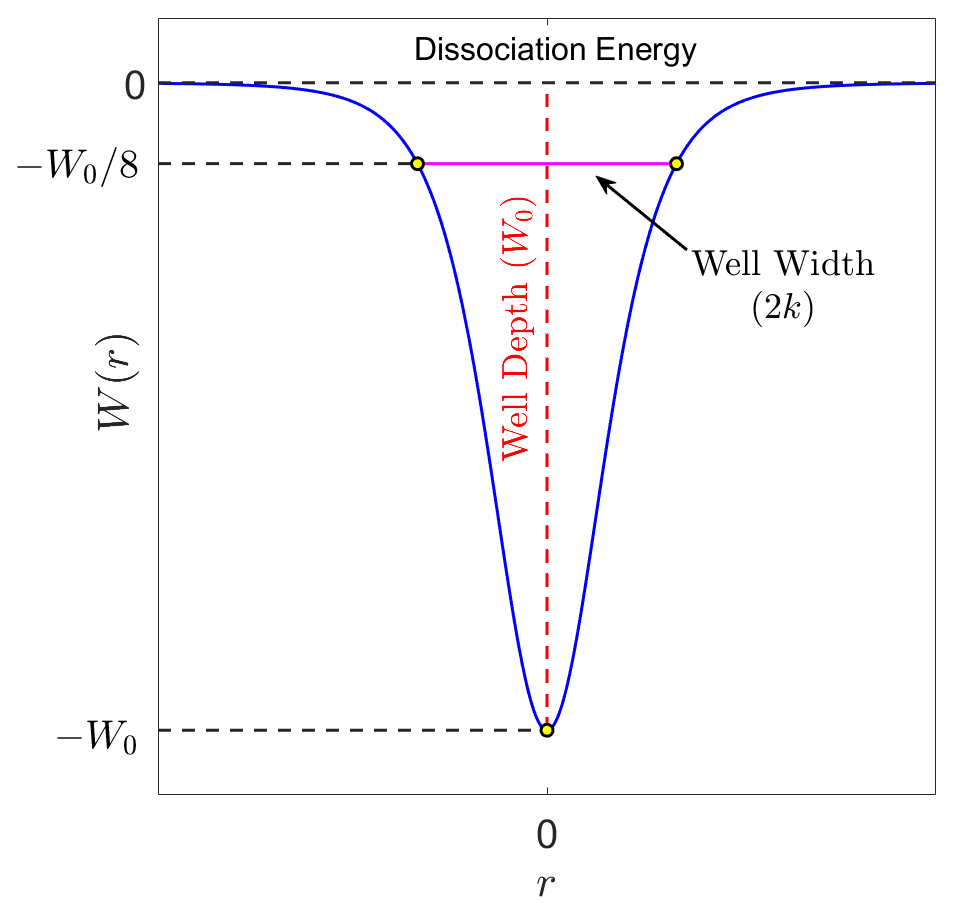
\includegraphics[scale=0.28]{heller_potFunc_new2.png}
	\caption{Geometrical interpretation of the parameters determining the shape of the PES in Eq. \eqref{eq:heller_pes}.}
	\label{fig:heller_pes}
\end{figure}


\begin{figure}[htbp]
	A)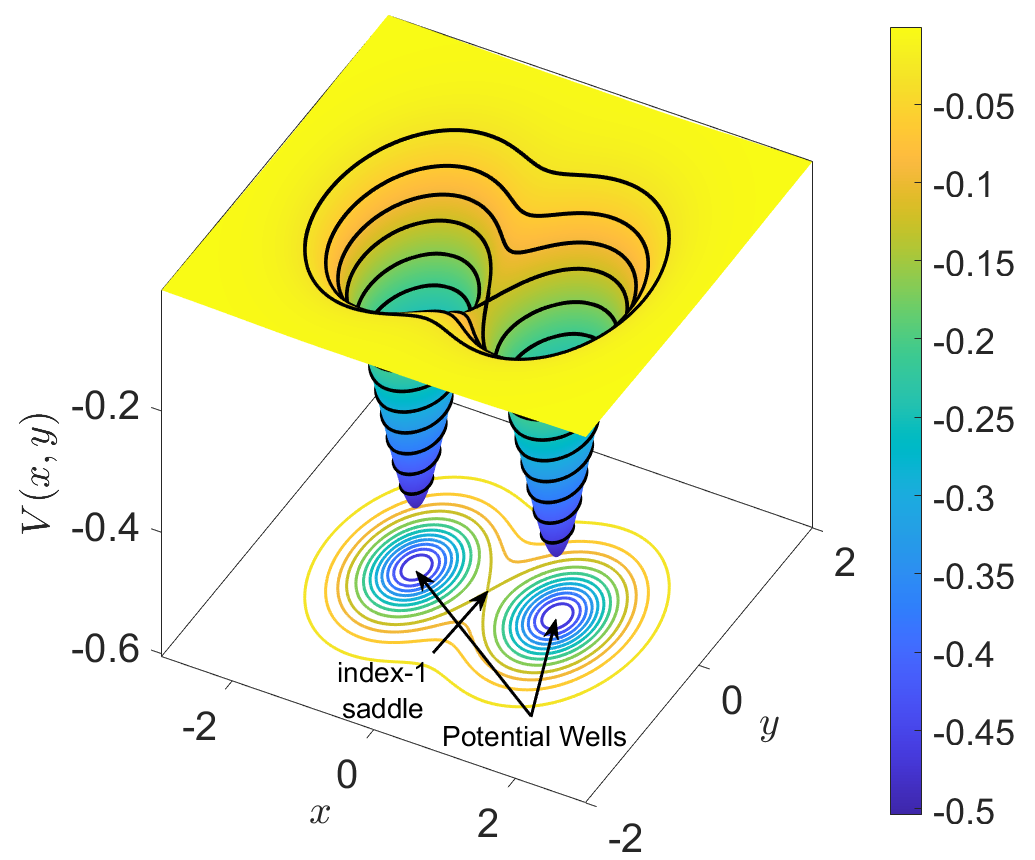
\includegraphics[scale=0.28]{PES_Cirque_w0_1div2_k_1_d_1.png}
	B)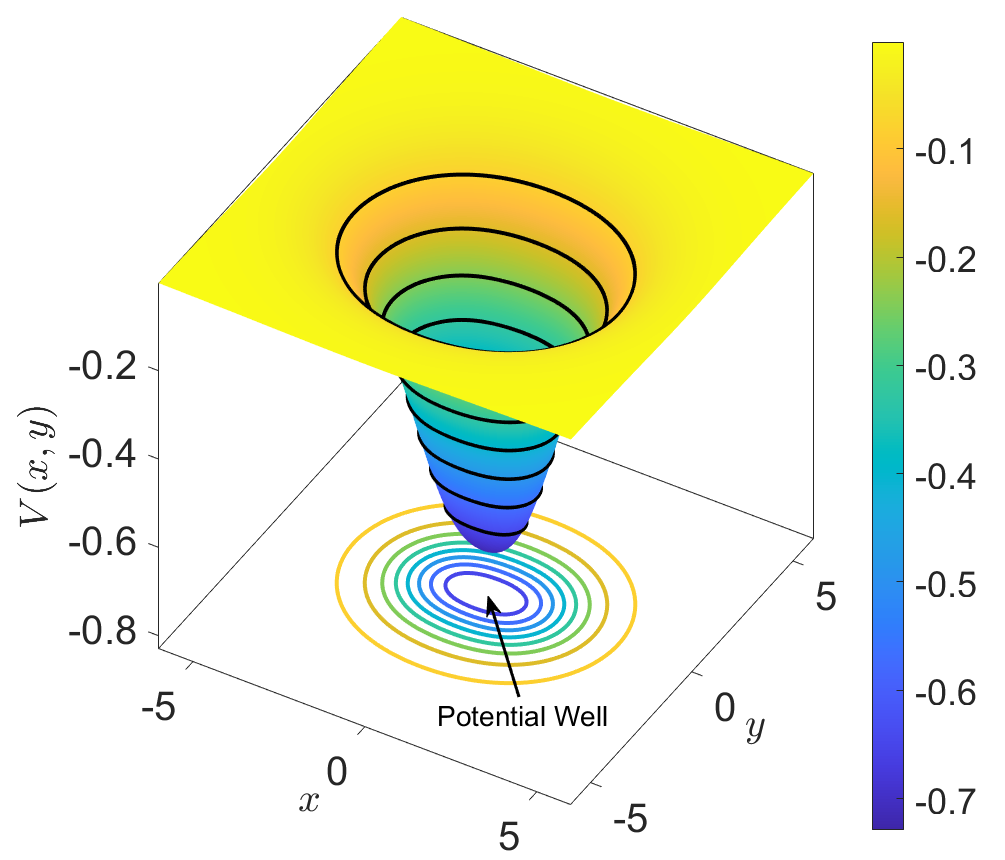
\includegraphics[scale=0.28]{PES_Cirque_w0_1div2_k_3_d_1.png}
	C)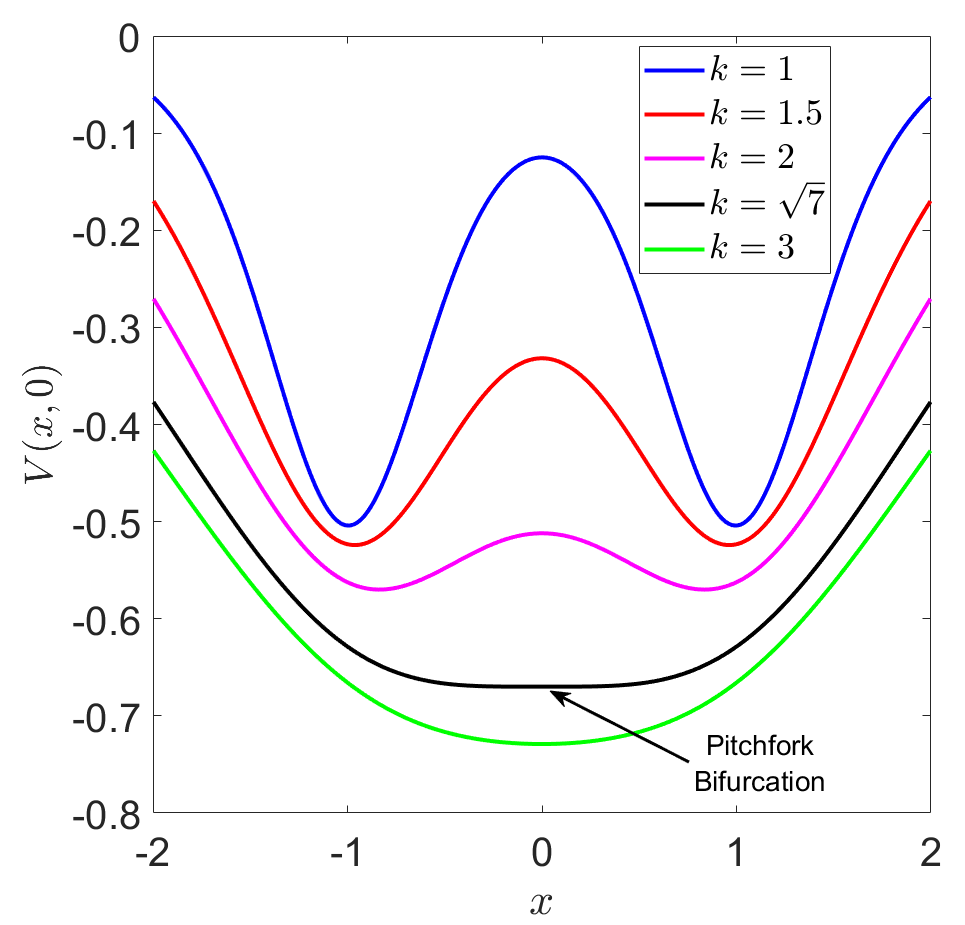
\includegraphics[scale=0.25]{pitcforkBif.png}
	\caption{Double van der Waals PES in Eq. \eqref{eq:double_vdw} for the model parameters: A) $W_0 = 1/2$, $k = 1$, $d = 1$; B) $W_0 = 1/2$, $k = 3$, $d = 1$; C) Pitchfork bifurcation of the PES along the $x$-axis for $W_0 = 1/2$ and $d = 1$, as the well width parameter $k$ is varied.}
	\label{fig:double_vdw_PES}
\end{figure}


%\begin{figure}[htbp]
%    A)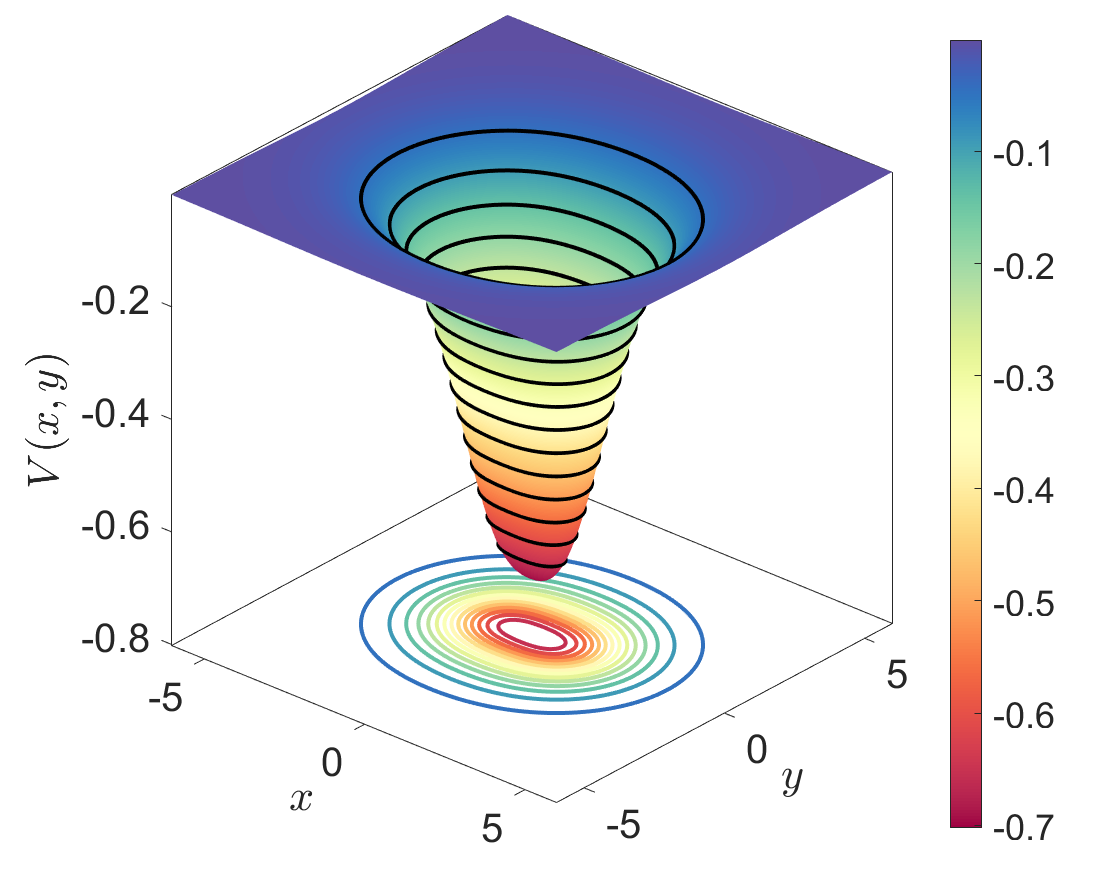
\includegraphics[scale=0.24]{CirquePES_c_1div2_a_1_b_1div8_d_1.png}
%    B)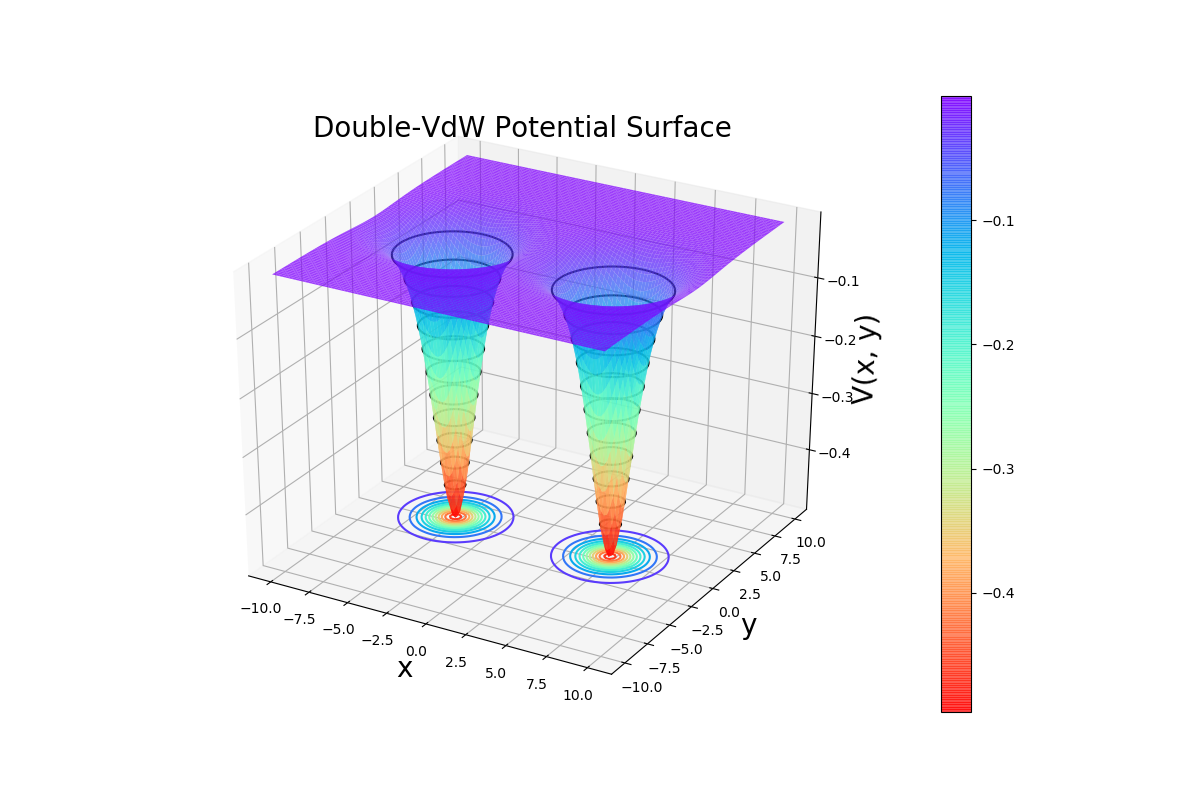
\includegraphics[scale=0.33]{double-vdw_surface.png}
%    \caption{Double van der Waals PES in Eq. \eqref{eq:vdw-single} for the model parameters: A) $C = 1/2$, $\alpha = 1$, $\beta = 1/8$ and $d = 1$; B) $C = 1/2$, $\alpha = 1$, $\beta = 1/8$, and $d = 5$.}
%    \label{fig:vdw-single_surface}
%\end{figure}

The two degrees-of-freedom (DoF) Hamiltonian for the Cirque potential energy surface is defined as the classical sum of kinetic plus potential energy:
\begin{equation}
H(x,y,p_x,p_y) = \dfrac{p_x^2}{2 m_1} + \dfrac{p_y^2}{2 m_2} + V(x,y)
\label{eq:hamil}
\end{equation}
where $m_1$ and $m_2$ are the masses in the $x$ and $y$ DoF respectively. Hamilton's equations that determine the systems dynamical evolution are given by:
\begin{equation}
\begin{cases}
\dot{x} = \dfrac{\partial H}{\partial p_x} = \dfrac{p_x}{m_1} \\[.5cm]
\dot{y} = \dfrac{\partial H}{\partial p_y} = \dfrac{p_y}{m_2} \\
\dot{p}_x = - \dfrac{\partial H}{\partial x} = - \dfrac{\partial V}{\partial x} = - 6 W_0 \, k^6 \left[\dfrac{x - d}{\left(\left(x - d\right)^2 + y^2 + k^2\right)^4} + \dfrac{x + d}{\left(\left(x + d\right)^2 + y^2 + k^2\right)^4}\right] \\[.8cm]
\dot{p}_y = - \dfrac{\partial H}{\partial y} = - \dfrac{\partial V}{\partial y} = - 6 W_0 \, k^6 y \left[\dfrac{1}{\left(\left(x - d\right)^2 + y^2 + k^2\right)^4} + \dfrac{1}{\left(\left(x + d\right)^2 + y^2 + k^2\right)^4}\right]
\end{cases}
\label{eq:ham_eq}
\end{equation}
In this work we will consider the situation where both DoF have unit mass, that is $m_1 = m_2 = 1$. The equilibrium points $\mathbf{x}_e = (x_e,y_e,p_{x,e},p_{y,e})$ of the dynamical system given above are contained in configuration space, since $p_{x,e} = p_{y,e} = 0$, and they are also critical points of the PES, that is $\nabla V (x_e,y_e) = \mathbf{0}$. It is straightforward to check that under these conditions, the points have to satisfy:
\begin{equation}
y_e = 0 \quad , \quad \left(x_e - d\right) \left[\left(x_e + d\right)^2 + k^2\right]^4 + \left(x_e + d\right) \left[\left(x_e - d\right)^2 + k^2\right]^4 = 0 
\label{eq:eq_pts}
\end{equation}
It is straightforward to show that $x_e = 0$ is always a solution to the equation above, and therefore the origin is always an equilibrium point of Hamilton's equations for this system. Moreover, there is also an equilibrium point located at infinity. Regarding the presence of other equilibria, this depends critically on the model parameters, and if they exist, their coordinates are of the form $\mathbf{x}_e = (x_e(k,d),0,0,0)$. 

The linear stability of these equilibrium points is determined by the eigenvalues of the Jacobian matrix given by the linearization of Eq. \eqref{eq:ham_eq} about each of the points. In order to construct the Jacobian, we need to compute the second order partial derivatives that characterize the Hessian matrix of the PES:
\begin{equation}
\begin{cases}
\dfrac{\partial^{\,	2} V}{\partial x^2} = 6 \, W_0 \, k^6 \left[\dfrac{-7\left(x - d\right)^2 + y^2 + k^2}{\left(\left(x - d\right)^2 + y^2 + k^2\right)^5} + \dfrac{-7\left(x + d\right)^2 + y^2 + k^2}{\left(\left(x + d\right)^2 + y^2 + k^2\right)^5} \right] \\[.8cm]

\dfrac{\partial^{\,	2} V}{\partial y^2} = 6 \, W_0 \, k^6 \left[\dfrac{\left(x - d\right)^2 - 7 y^2 + k^2}{\left(\left(x - d\right)^2 + y^2 + k^2\right)^5} + \dfrac{\left(x + d\right)^2 - 7y^2 + k^2}{\left(\left(x + d\right)^2 + y^2 + k^2\right)^5} \right] \\[.8cm]

\dfrac{\partial^{\,	2} V}{\partial x \partial y} = - 48 \, W_0 \, k^6 \, y \left[\dfrac{x - d}{\left(\left(x - d\right)^2 + y^2 + k^2\right)^5} + \dfrac{x + d}{\left(\left(x + d\right)^2 + y^2 + k^2\right)^5}\right]
\end{cases}
\label{eq:second_pder}
\end{equation}
We take a look now at the Hessian matrix of the PES evaluated at the origin:
\begin{equation}
\text{Hess}_{V}(0,0) = \begin{pmatrix}
\dfrac{\partial^{\,	2} V}{\partial x^2}(0,0) & \dfrac{\partial^{\,	2} V}{\partial x \partial y}(0,0) \\[.4cm]
\dfrac{\partial^{\,	2} V}{\partial y \partial x}(0,0) & \dfrac{\partial^{\, 2} V}{\partial y^2}(0,0)
\end{pmatrix} = \begin{pmatrix}
\dfrac{12 W_0 \, k^6 \left(k^2 - 7 d^2\right)}{\left(d^2 + k^2\right)^5} & 0 \\[.5cm]
0 & \dfrac{12 W_0 \, k^6}{\left(d^2 + k^2\right)^4}
\end{pmatrix}
\end{equation}
The linear stability of the origin is characterized by the nature of the eigenvalues of the Jacobian matrix:
\begin{equation}
J(0,0) = \begin{pmatrix}
\mathbb{O}_2 & \hspace{.2cm} \mathbb{I}_2 \hspace{.1cm} \\[.3cm]
-\text{Hess}_{V}(0,0) & \hspace{.2cm} \mathbb{O}_2 \hspace{.1cm}
\end{pmatrix} = \begin{pmatrix}
0 & 0 & \hspace{.5cm} 1 & \hspace{.5cm} 0 \hspace{.2cm} \\[.4cm]
0 & 0 & \hspace{.5cm} 0 & \hspace{.5cm} 1 \hspace{.2cm} \\[.4cm]
\dfrac{12 W_0 \, k^6 \left(7 d^2 - k^2\right)}{\left(d^2 + k^2\right)^5} & 0 & \hspace{.5cm} 0 & \hspace{.5cm} 0 \hspace{.2cm} \\[.4cm]
0 & -\dfrac{12 W_0 \, k^6}{\left(d^2 + k^2\right)^4} & \hspace{.5cm} 0 & \hspace{.5cm} 0 \hspace{.2cm} 
\end{pmatrix}
\end{equation}
The eigenvalues $\xi$ are given by:
\begin{equation}
\xi_{1,2} = \pm \, \omega \, i \quad,\quad \xi_{3,4} = \pm \, \omega \, \sqrt{\dfrac{7 d^2 - k^2}{ d^2 + k^2}} = \pm \, \omega \, \sqrt{\dfrac{7 -  \eta^2}{1 + \eta^2}}
 \end{equation}
where $\eta = k / d$ is the ratio between the half-width of the single van der Waals potential and its displacement from the origin, and the angular frequency of oscillation in the linear approximation is:
\begin{equation}
\omega = 2 \, \sqrt{3 W_0}\dfrac{k^3}{\left(d^2 + k^2\right)^2} = 2 \, \sqrt{\dfrac{3 W_0}{k^2}} \dfrac{\eta^4}{\left(1 + \eta^2\right)^2}
\end{equation}
Therefore, the origin is an index-1 saddle equilibrium point when the condition $7 d^2 \geq k^2$ is met, which is equivalent to $0 < \eta < \sqrt{7}$. However, for $\eta > \sqrt{7}$ the index-1 saddle turns into a potential well (a center equilibrium point). This indicates that there is a pitchfork bifurcation taking place in the PES at the origin at the critical relation $\eta = \sqrt{7}$. We illustrate this behavior in Fig. \ref{fig:double_vdw_PES} C) by looking at how the shape of the PES changes along the $x$-axis.





\section{Results}
\label{sec:results}


\begin{figure}[htbp]
	A)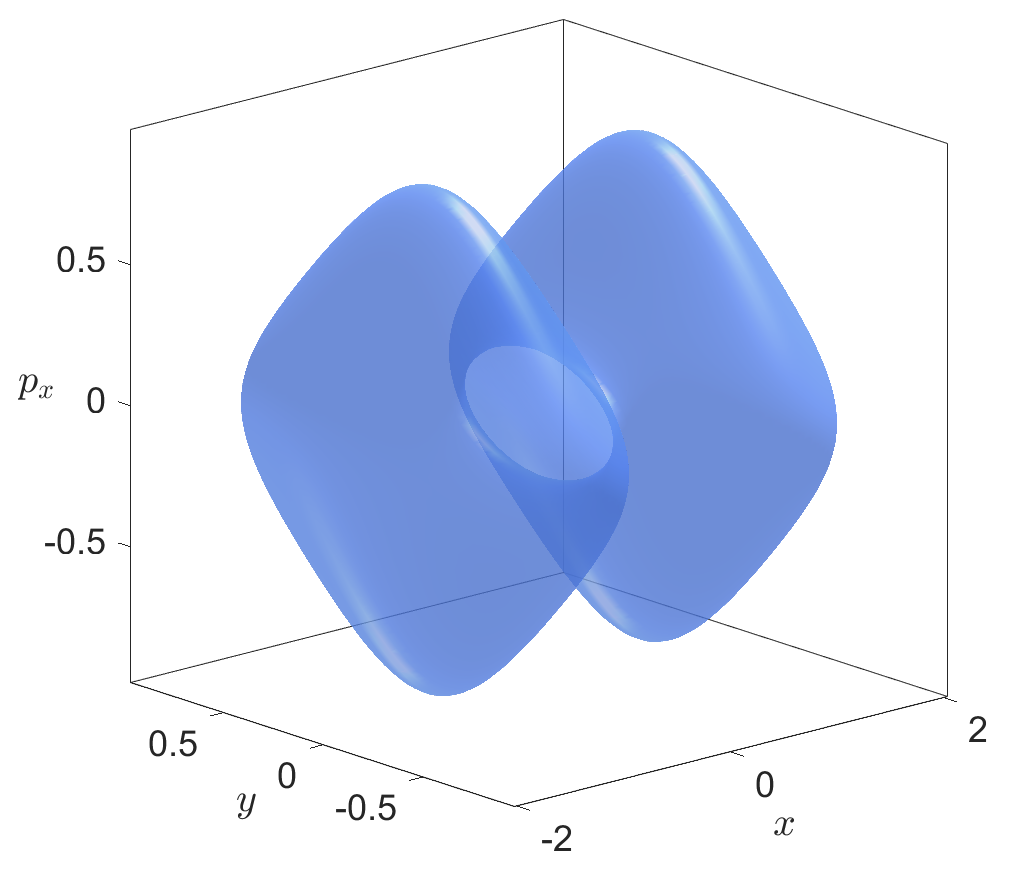
\includegraphics[scale=0.28]{energySurf_H_-01.png}
	B)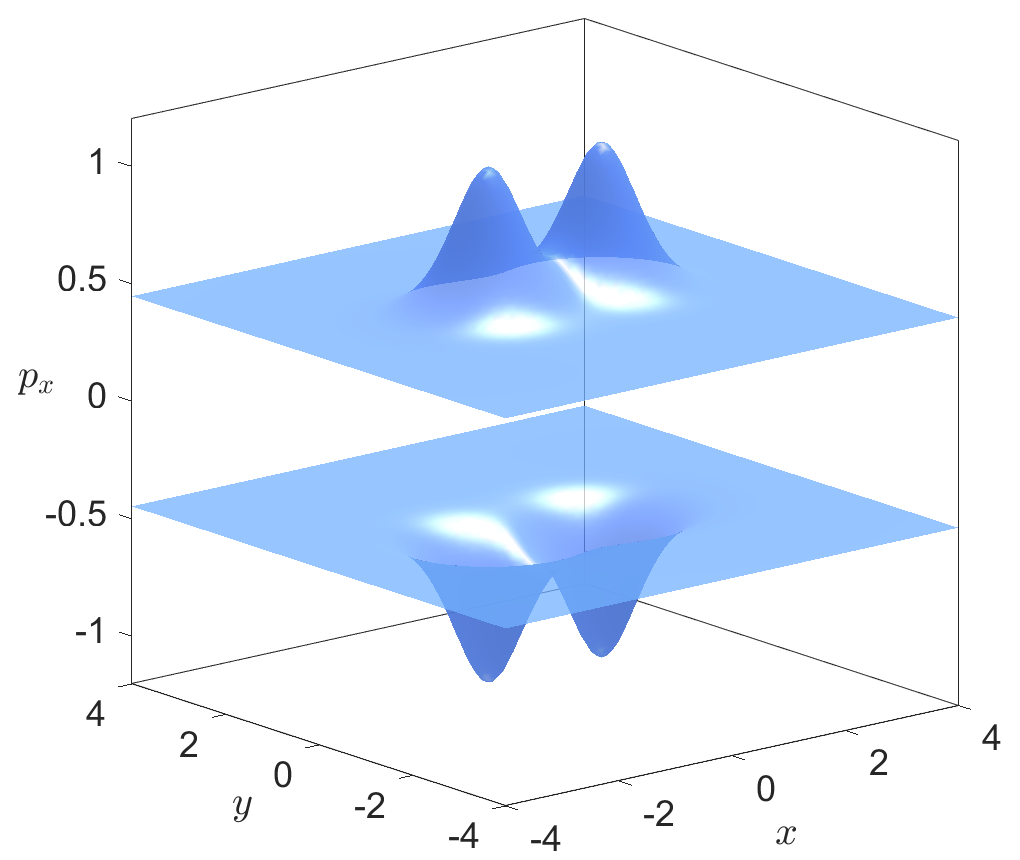
\includegraphics[scale=0.28]{energySurf_H_01.png}
	\caption{$W_0 = 1/2$ and $k = 1$. A) $H_0 = -0.1$; B) $H_0 = 0.1$.}
	\label{fig:vdw-energyHyp}
\end{figure}

\begin{figure}[htbp]
	A)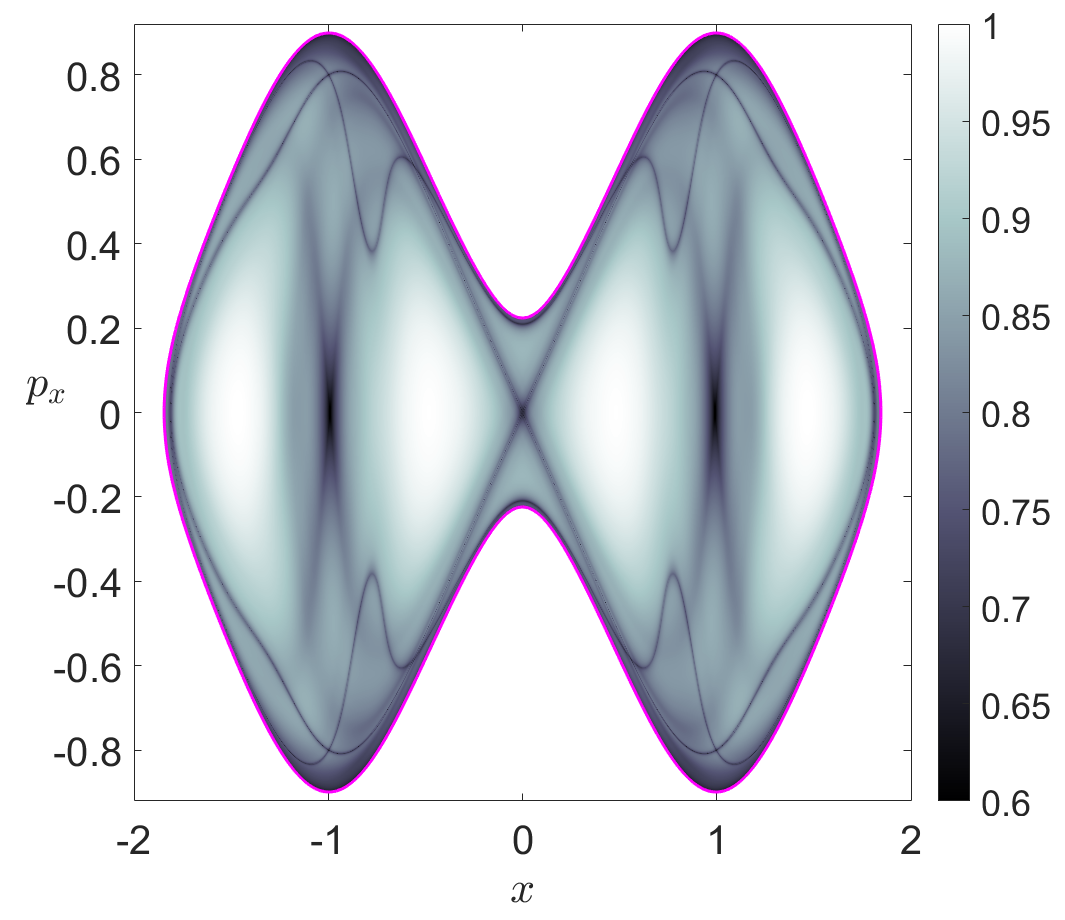
\includegraphics[scale=0.28]{H_-01_LD_tau_12_y_0.png}
	B)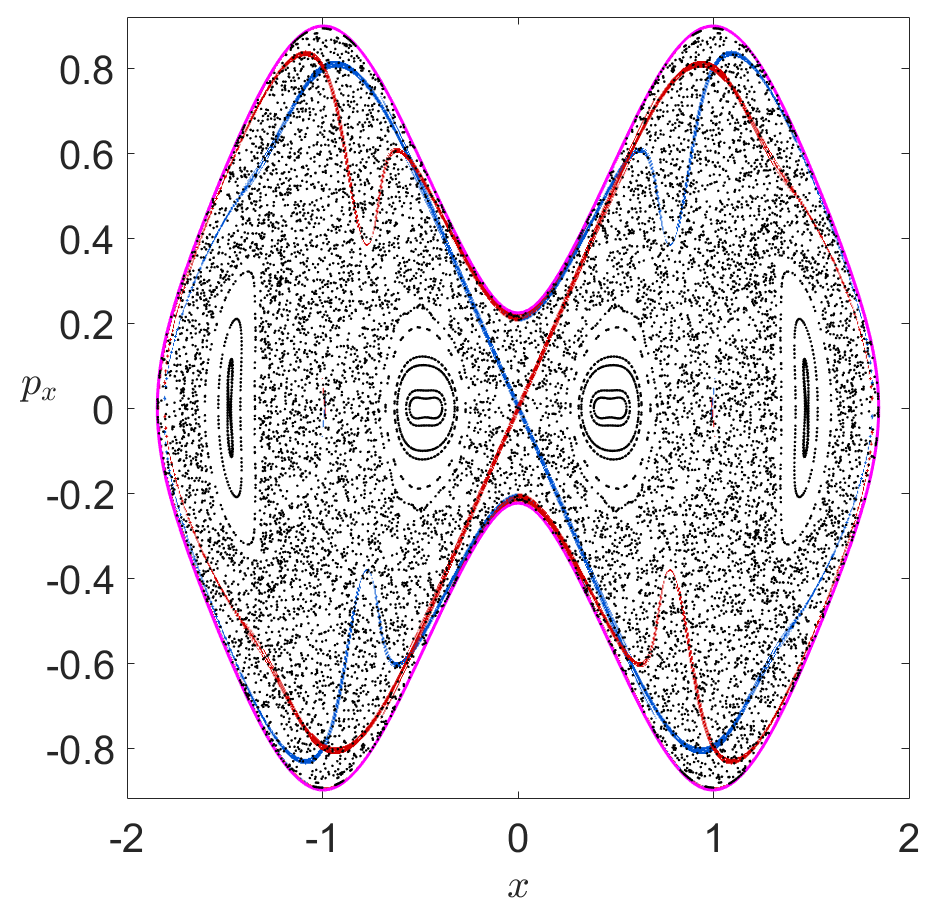
\includegraphics[scale=0.28]{H_-01_mani_tau_12_y_0.png}	
	C)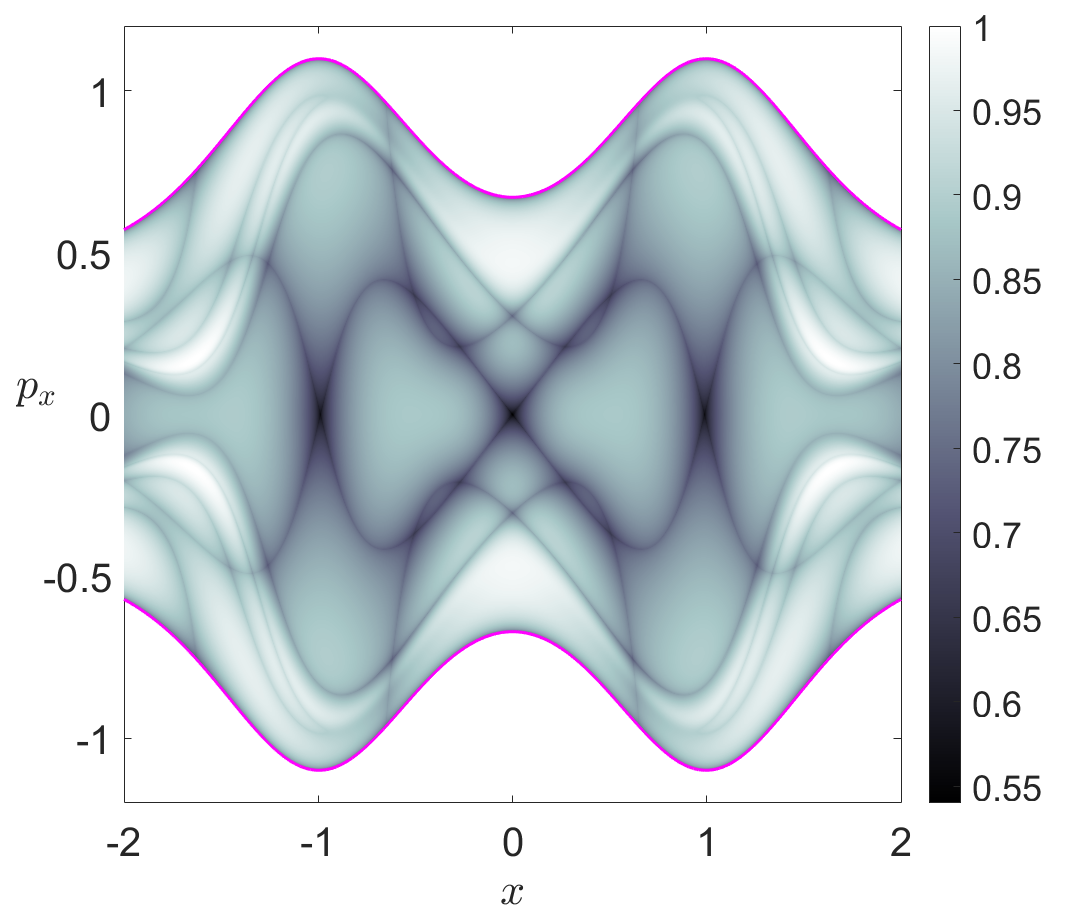
\includegraphics[scale=0.28]{H_01_LD_tau_12_y_0.png}
	D)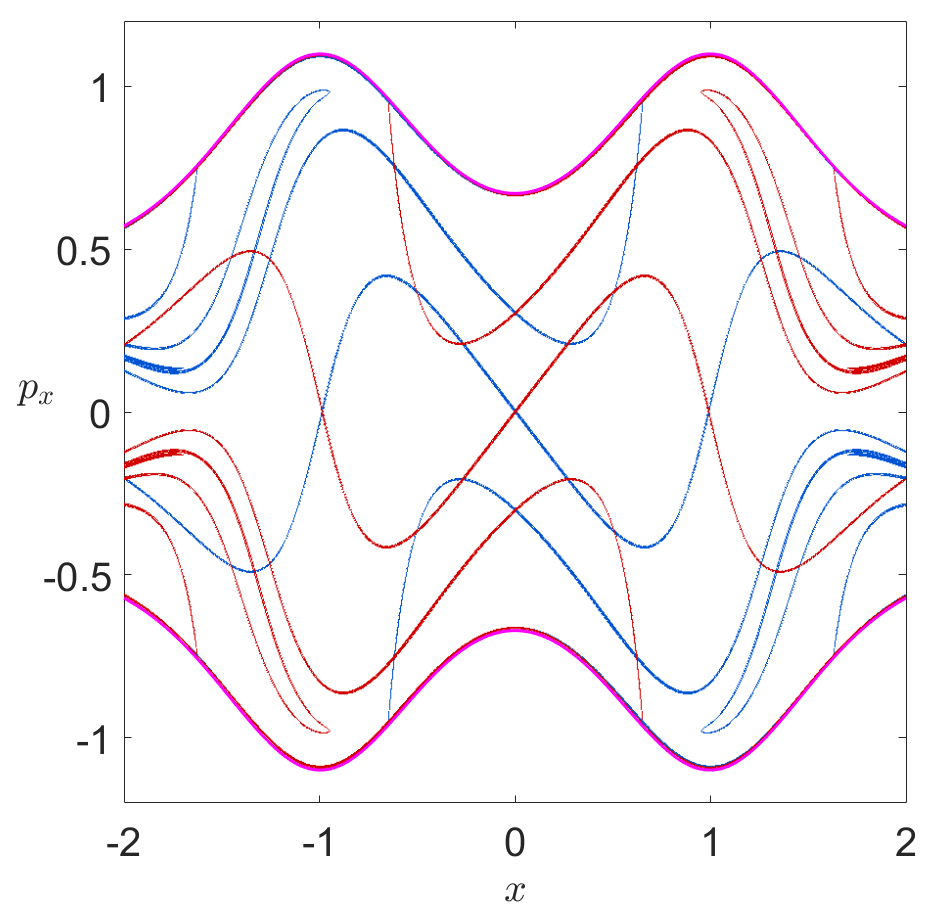
\includegraphics[scale=0.28]{H_01_mani_tau_12_y_0.png}
	\caption{Parameters $W_0 = 1/2$ and $k = 1$. Poincar\'e section $y = 0$. Top row energy $H_0 = -0.1$. Bottom row energy $H_0 = 0.1$.}
	\label{fig:ld_mani_y_0}
\end{figure}

\begin{figure}[htbp]
	A)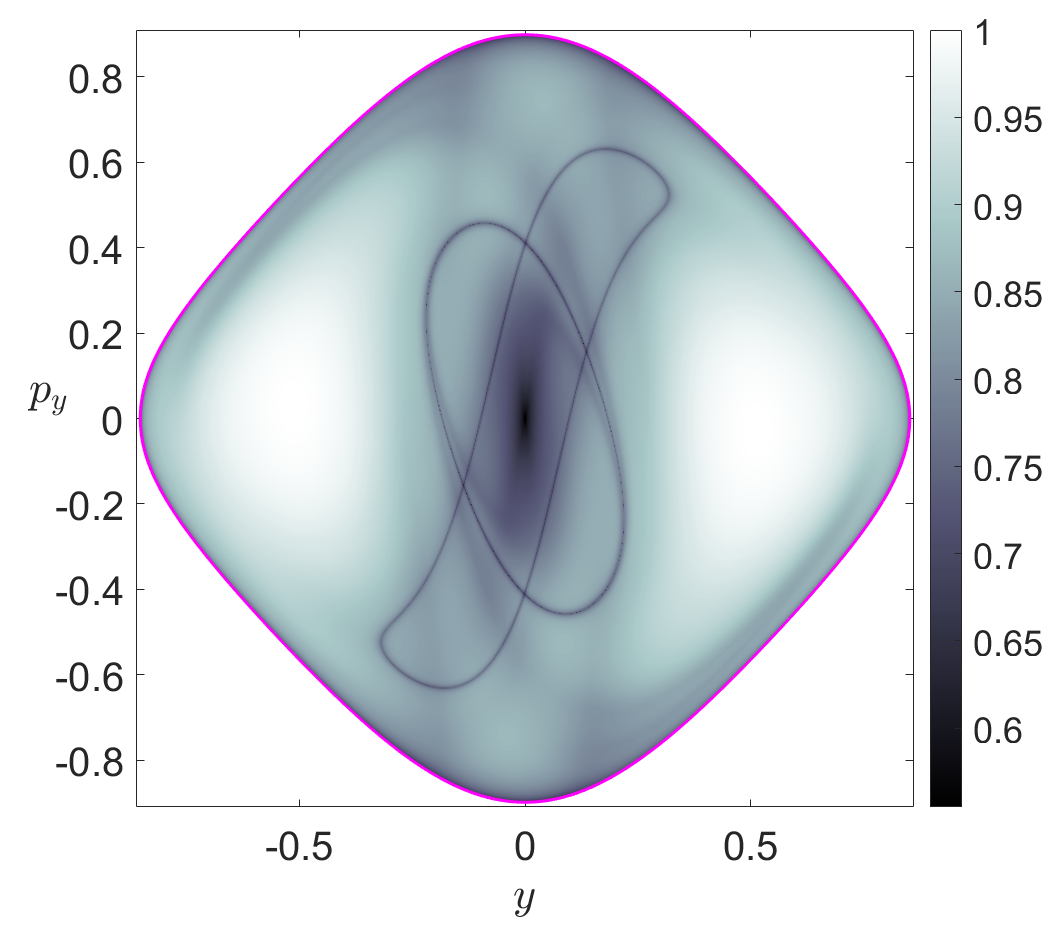
\includegraphics[scale=0.28]{H_-01_LD_tau_12_x_1.png}
	B)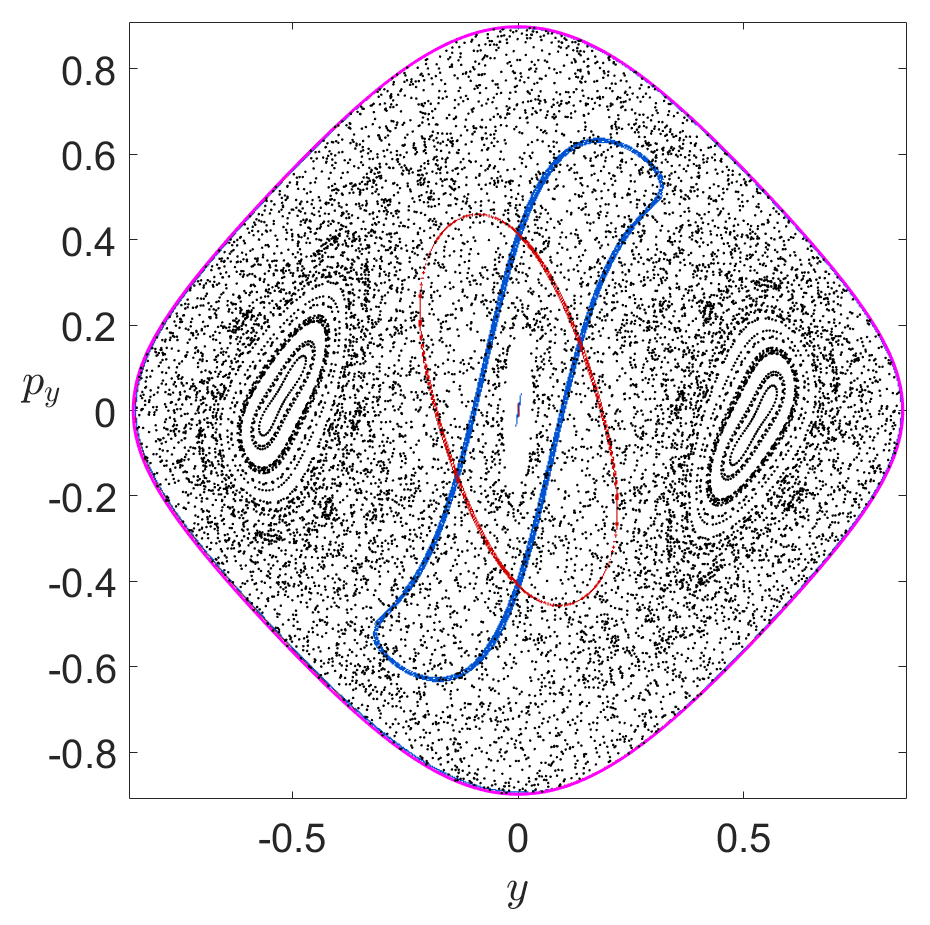
\includegraphics[scale=0.28]{H_-01_mani_tau_12_x_1.png}	
	C)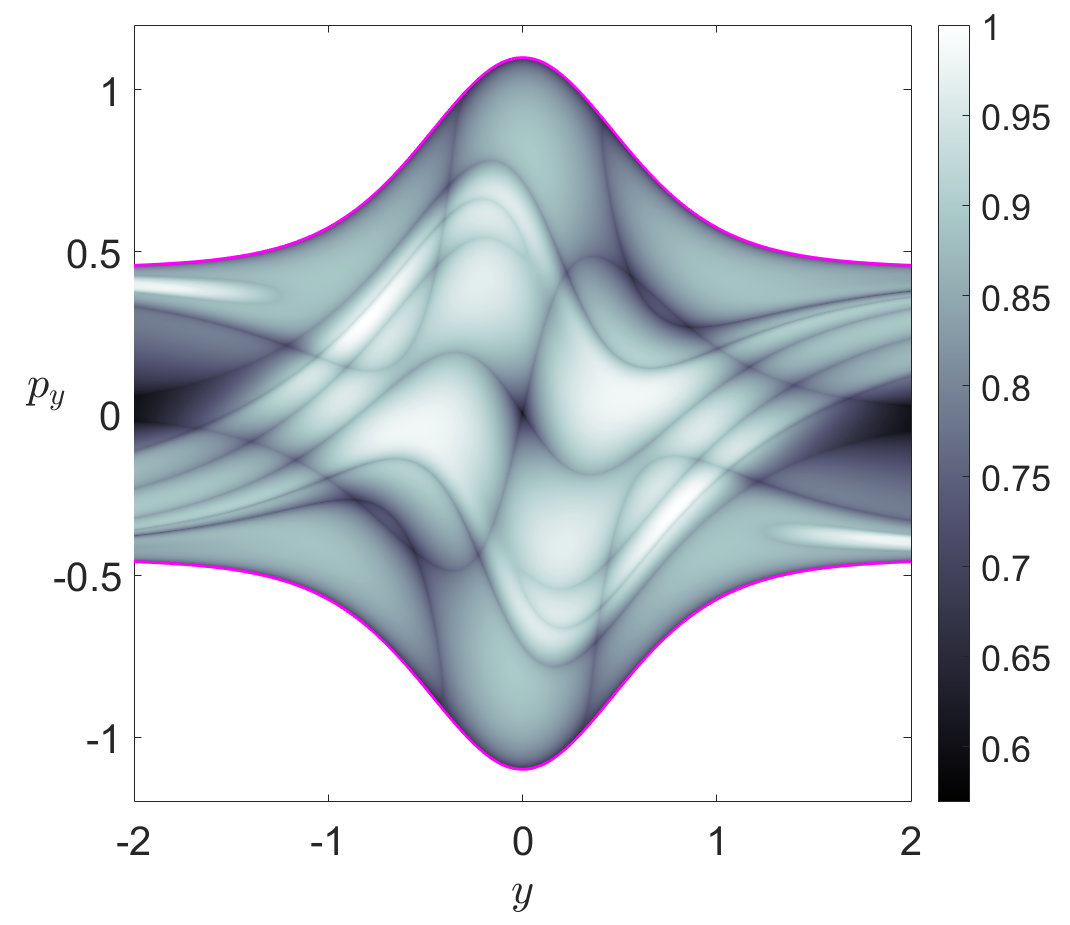
\includegraphics[scale=0.28]{H_01_LD_tau_12_x_1.png}
	D)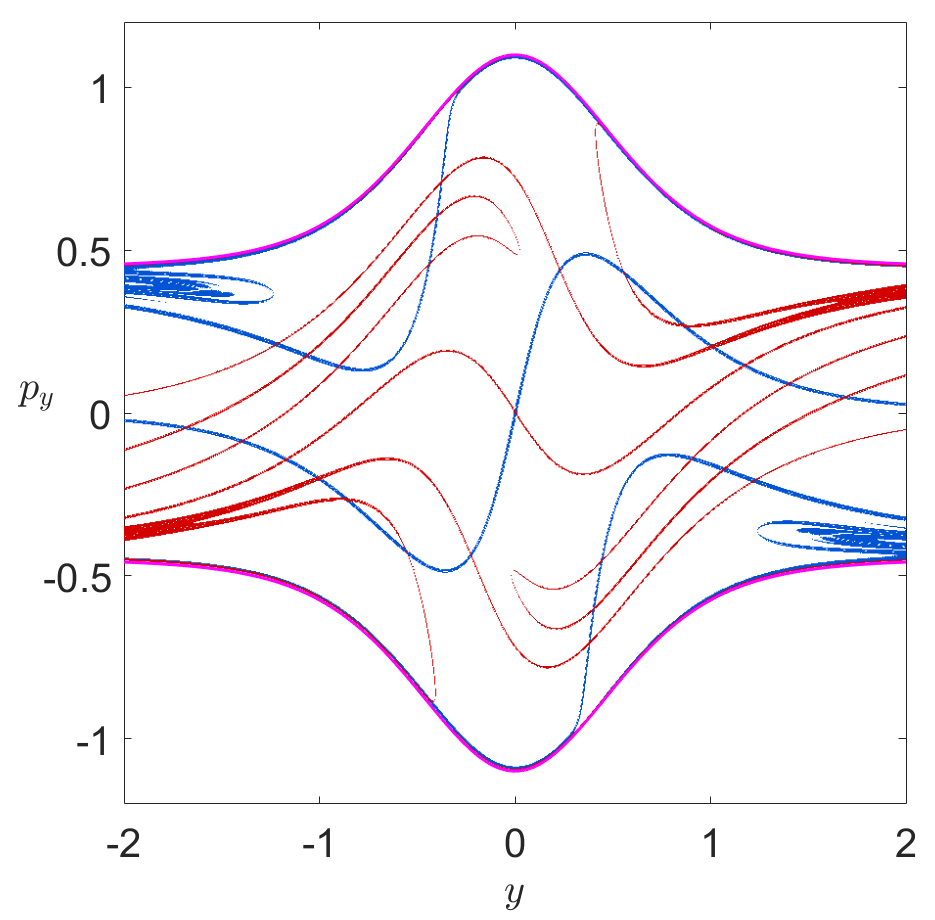
\includegraphics[scale=0.28]{H_01_mani_tau_12_x_1.png}
	\caption{Parameters $W_0 = 1/2$ and $k = 1$. Poincar\'e section $x = 1$. Top row energy $H_0 = -0.1$. Bottom row energy $H_0 = 0.1$.}
	\label{fig:ld_mani_x_1}
\end{figure}

\begin{figure}[htbp]
	A)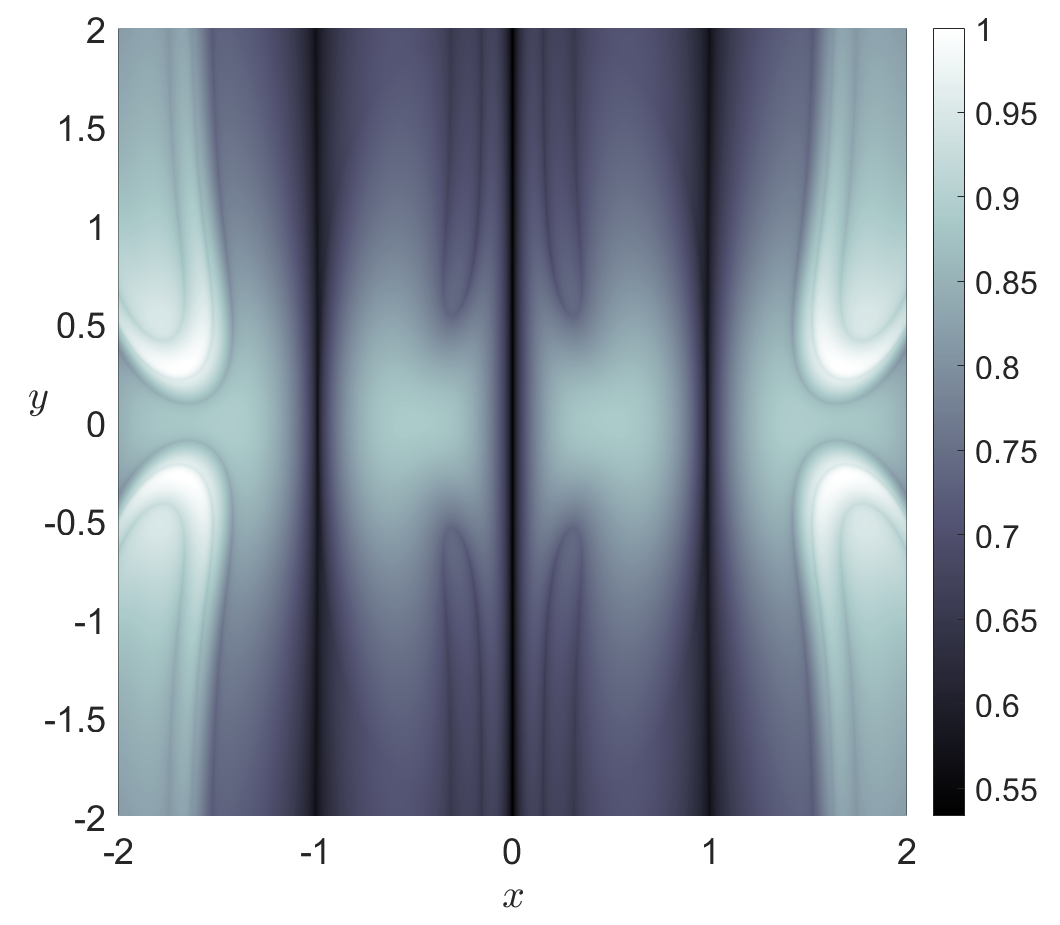
\includegraphics[scale=0.28]{H_01_LD_tau_12_px_0.png}
	B)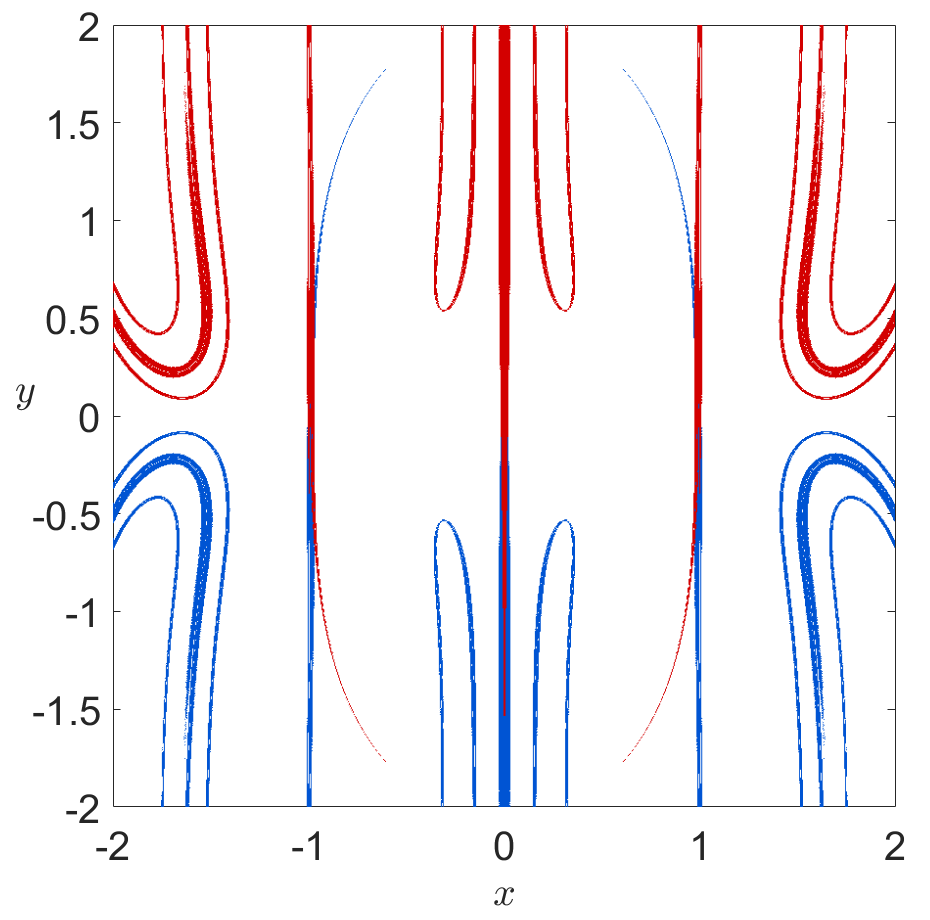
\includegraphics[scale=0.28]{H_01_mani_tau_12_px_0.png}	
	\caption{Parameters $W_0 = 1/2$ and $k = 1$. Poincar\'e section $p_x = 0$. Energy $H_0 = 0.1$.}
	\label{fig:ld_mani_px_0}
\end{figure}



%%%%%%%%%%%%%%%
\newpage

\subsection{ $E>0$ Transport between potential wells and Roaming }


In this section, we study the transport associated with the roaming phenomenon. This potential energy $V(x,y)$ has some common features with the other potential energies surfaces where the roaming has been observed. The potential energy has two wells and a region where it is almost flat and its value goes to zero \ref{fig:double_vdw_PES}. For energies $E$ > 0 the phase space of the system becomes unbounded and the trajectories can escape from the potential wells. The Lagrangian descriptor plots in figure \ref{fig:ld_x_px} show how the structure of the phase space change when the goes from negative to positive. A trajectory presents roaming phenomenon if the particle travels from one potential well to the other one visiting the region where the potential energy surface is almost flat. This behaviour is associated with a special kind of chemical reaction where a molecule divide in two parts, then one part of the molecule travel around the other one before both parts recombine again and form a new molecule. This kind of reaction is impossible to explain if the motion of the fragments of the molecule is not considered. The roaming reaction happens only for a special combination of momentum and position of the reactants. 

Following a previous studies of roaming for the double Morse potential well \cite{Carpenter2017,Carpenter2018, GonzalezMontoya2020}, let us consider the trajectories that go from one potential well to the other potential well and the trajectories that go from one potential well to the asymptotic region. To carry out this study let us consider 3 regions in the configuration space: 2 circles with the same radius, whose centres are close to the minimum of each potential well, regions $A$ and $B$, and a circle containing the two potential wells whose border is in the asymptotic region $C$, where the particle is almost a free particle. In the next numerical example, the radii that define the regions $A$, $B$, and $C$ are 1.5 and 5.0 respectively.

In the double Morse system, there are three families of unstable hyperbolic periodic orbits that control the roaming. To define the families of periodic orbits, let us consider their projection on the configuration space. The projection of the first family of periodic orbits encircle both potential wells, the projection of the second family of periodic orbits encircle both potential wells and crosses the origin, and the projection of the periodic orbits corresponding to the third family encircle one well. In the present system, the same kind of periodic orbits exist for energies close to the threshold energy $E>0$, see figures \ref{fig:periodic_orbits_roaming}. Using Lagrangian descriptors or other chaos indicator we can find the values of $E$ where these families of hyperbolic periodic orbits exist  \cite{Demian2017,Gonzalez2020}. The stable and unstable manifolds of the hyperbolic periodic orbits generate singularities on the Lagrangian descriptor plots.

In order to find the values of $E$ where the hyperbolic periodic orbit bifurcate, we calculate the Lagrangian descriptor on a set of initial conditions that contains the periodic orbits as a function of the $E$. In this particular example, a member of each family of hyperbolic periodic orbits crosses the line $y_0=0$ with momentum $p_{x0}$ = 0, see figure \ref{fig:periodic_orbits_roaming}. The Lagrangian descriptor corresponding to this set of initial conditions is in the figure \ref{fig:ld_E_xy}. The maxima around the points  $(E,x_0)$ = $(2.144,0.019)$, $(1.920,0.029)$, and $(1.678,0.659)$ on this figure corresponds to the energies of the bifurcation and the point where the periodic orbits intersect the $x_0$ axis. 


\begin{figure}[htbp]
	A)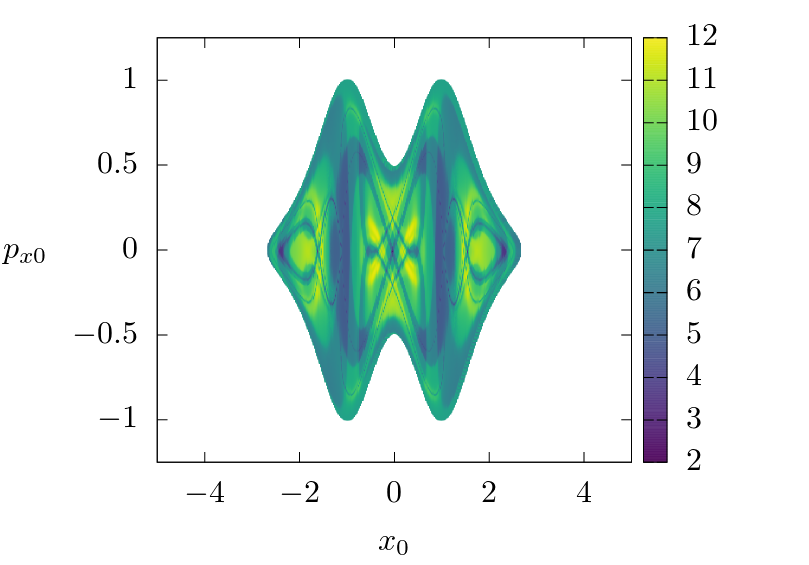
\includegraphics[scale=0.35]{ld_xpx_t20_E-001.png}
	B)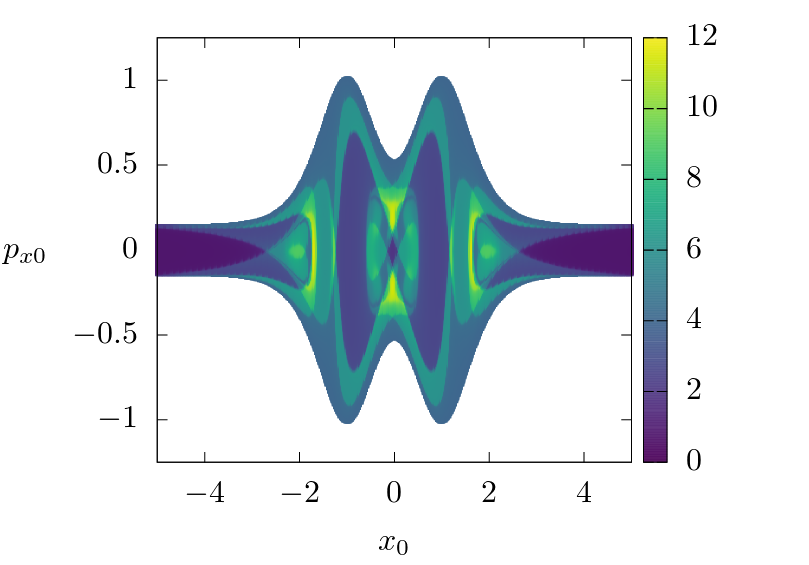
\includegraphics[scale=0.35]{ld_xpx_t20_E001.png}	
	\caption{Lagrangian descriptors plots based on the action $S_0$ for $E =-0.01$ and $0.01$. The initial momentum has $p_{y0}=0$ and the integration time $\tau=20$ ($W_0 = 1/2$ and $k = 1$). For energies $E > 0$ the phase space becomes unbounded and the trajectories can escape to infinity. On the figure B) the periodic orbit $\Gamma_1$ is created, their stable and unstable manifolds intersect the plane  around  $(x_0,p_{x0})=(2.6,0)$ }
	\label{fig:ld_x_px}
\end{figure}


\begin{figure}[htbp]
	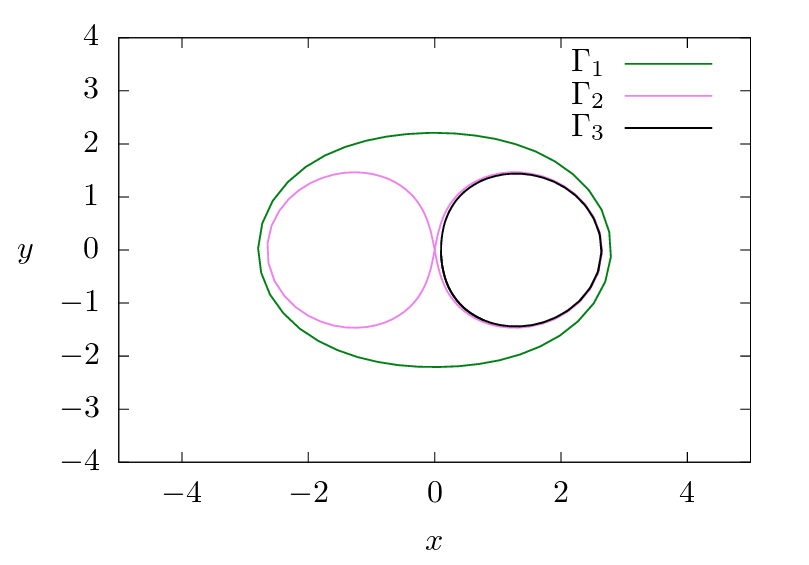
\includegraphics[scale=0.5]{orbits_2D.png}
	\caption{ Hyperbolic periodic orbits $\Gamma_1$, $\Gamma_2$, and $\Gamma_3$ associated with the roaming in the configuration space. $E$ = 0.01. }
	\label{fig:periodic_orbits_roaming}
\end{figure}




\begin{figure}[htbp]
	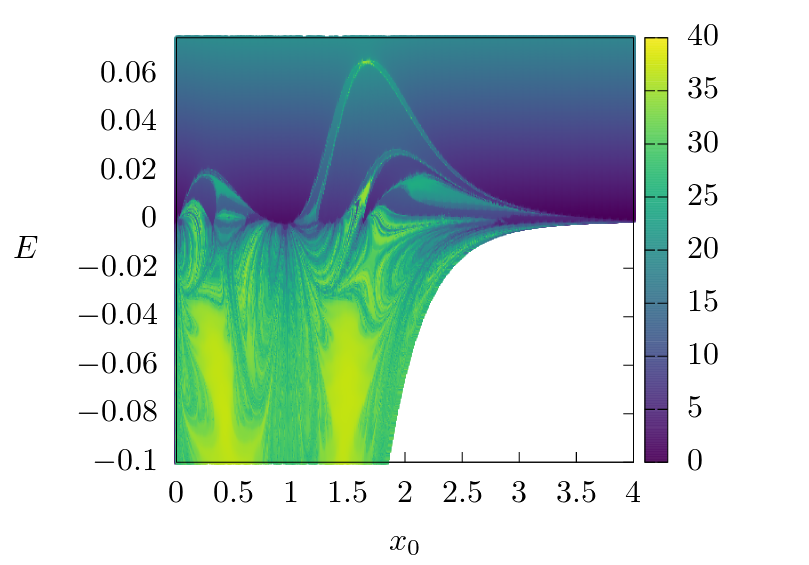
\includegraphics[scale=0.5]{ld_t60_line_x_E.png}
	%B)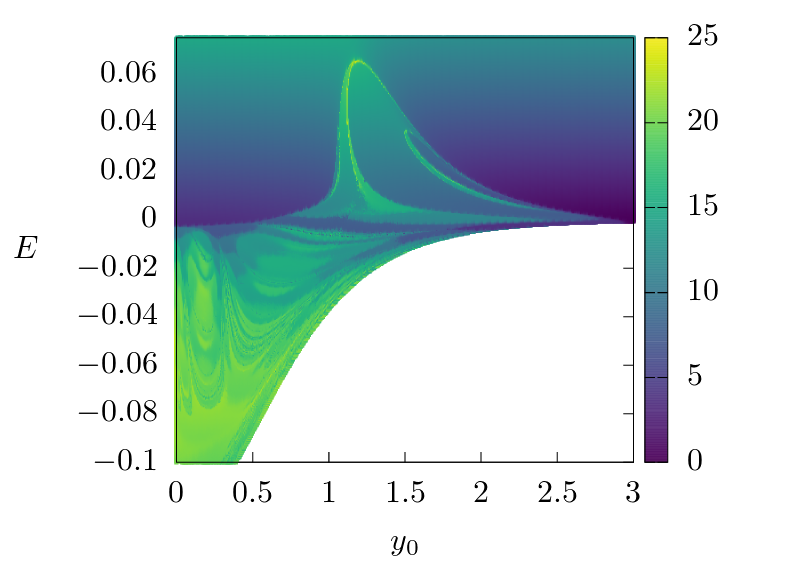
\includegraphics[scale=0.35]{ld_t60_line_y_E.png}
	\caption{Bifurcations diagrams based on Lagrangian descriptor $E$ vs $x_0$. The integration time $\tau=60$ ($W_0 = 1/2$ and $k = 1$.}
	\label{fig:ld_E_xy}
\end{figure}


In order to study the transport between the wells and the roaming, we consider the dividing surface associated with the periodic orbits $\Gamma_1$, $\Gamma_2$, and $\Gamma_3$. The dividing surface of one periodic orbit has 3 important properties:

\begin{itemize}
    \item The flux is minimal on the dividing surface
    \item The periodic orbits associated with the dividing surface are  subsets of the dividing surface.
    \item All the trajectories that cross the dividing surface crosses the projection of the periodic orbit.
\end{itemize}

The last property is important for our study of the transport between wells and roaming. We can visualise the regions with the same fate on the dividing surface.

The algorithm to construct the dividing surface of a periodic orbit consist of 3 steps:

\begin{itemize}
    \item Project the periodic orbit on the configuration space
    \item For each point $(x,y)$ on the configuration space construct the circle compatible with the conservation of the energy
    \[ p^2_x + p^2_y =  2m(E - V(x,y)) \]
    \item Take the union of all the circles for any point in the projection of the periodic orbit.
\end{itemize}

The next figures show the fate maps and the Lagrangian descriptor plots evaluated on the dividing surfaces for different values of the energy. We consider values of $E$ after and before the bifurcation of the periodic orbits. The boundaries of the regions with different fates correspond to singularities on the Lagrangian descriptor plots. The singularities are a characteristic signal of the presence of stable and unstable manifolds. The stable and unstable manifolds have 2 dimensions and direct the trajectories and divide the regions with different fates in the constant energy manifold.


\begin{figure}[htbp]
	A)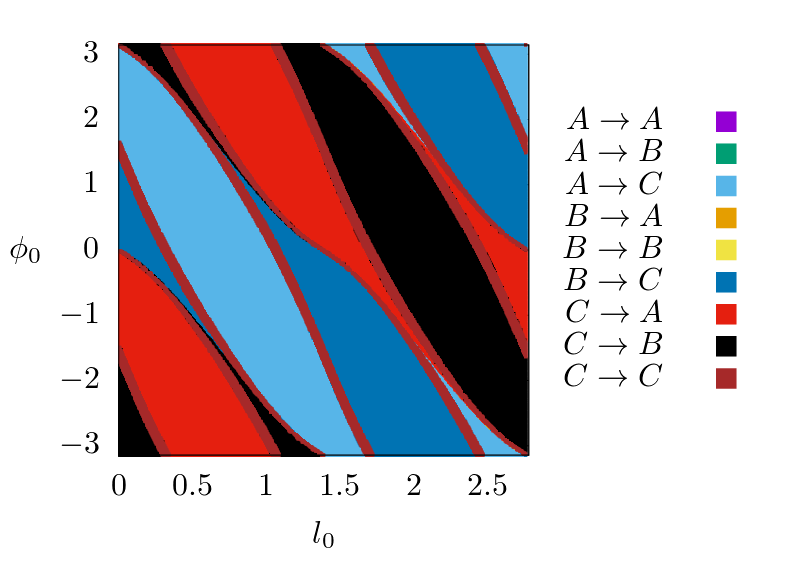
\includegraphics[scale=0.35]{fate_map_ds_gamma1E_001.png}
	B)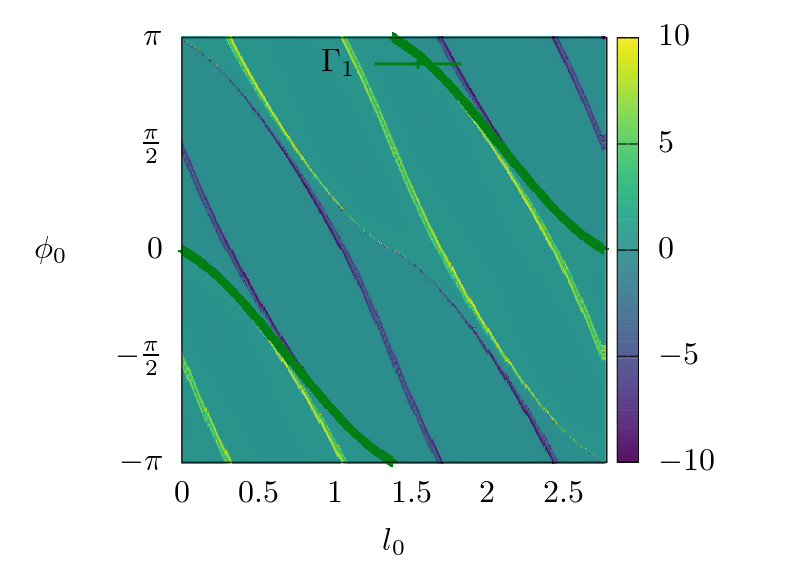
\includegraphics[scale=0.35]{ld_action_ds_gamma1_E_001.png}
	C)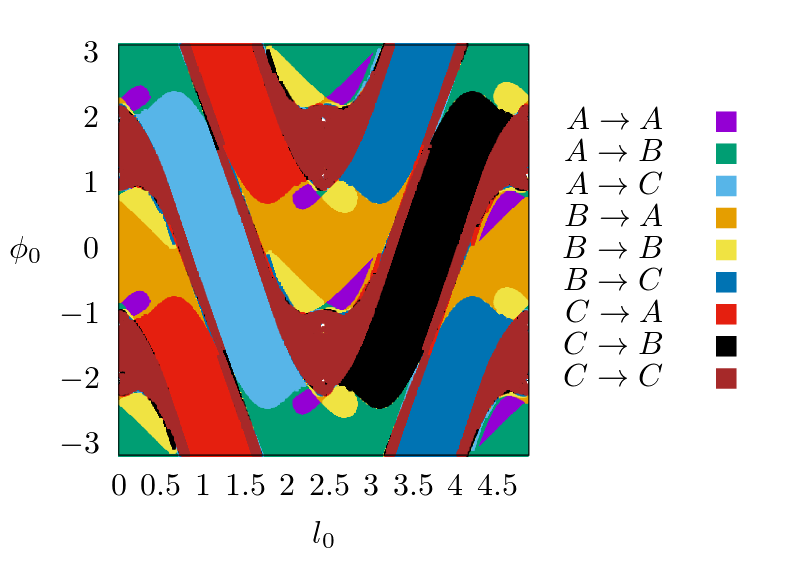
\includegraphics[scale=0.35]{fate_map_ds_gamma2E_001.png}
	D)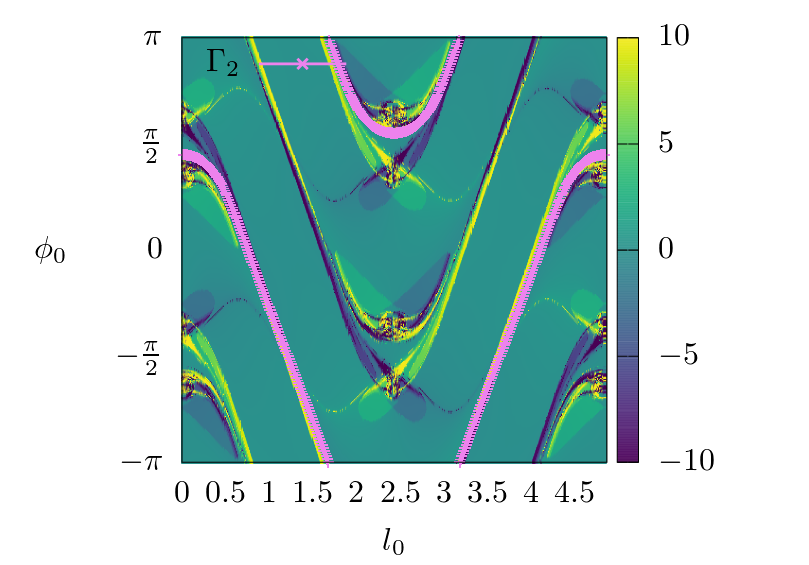
\includegraphics[scale=0.35]{ld_action_ds_gamma2_E_001.png}
	E)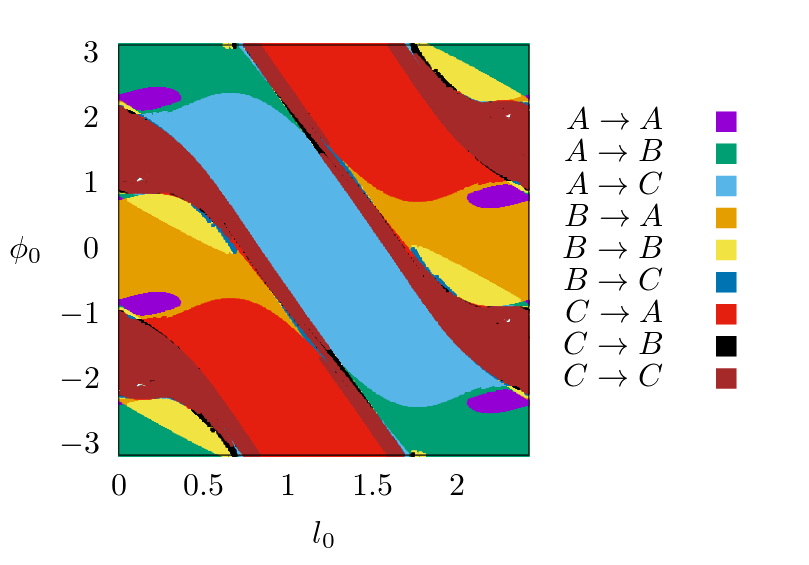
\includegraphics[scale=0.35]{fate_map_ds_gamma3E_001.png}
	F)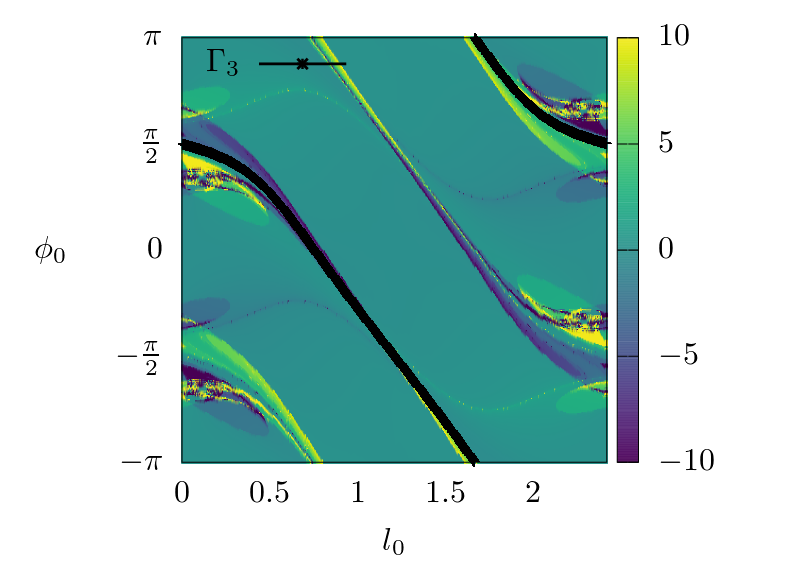
\includegraphics[scale=0.35]{ld_action_ds_gamma3_E_001.png}
	\caption{ Fate maps and Lagrangian descriptors evaluated on the dividing surface corresponding to periodic orbits $\Gamma_1$, $\Gamma_2$, and $\Gamma_3$ for an energy close to the dissociation threshold ($E$ =0.01). }
	\label{fig:ld_fm_ds_E_001}
\end{figure}





\begin{figure}[htbp]
	A)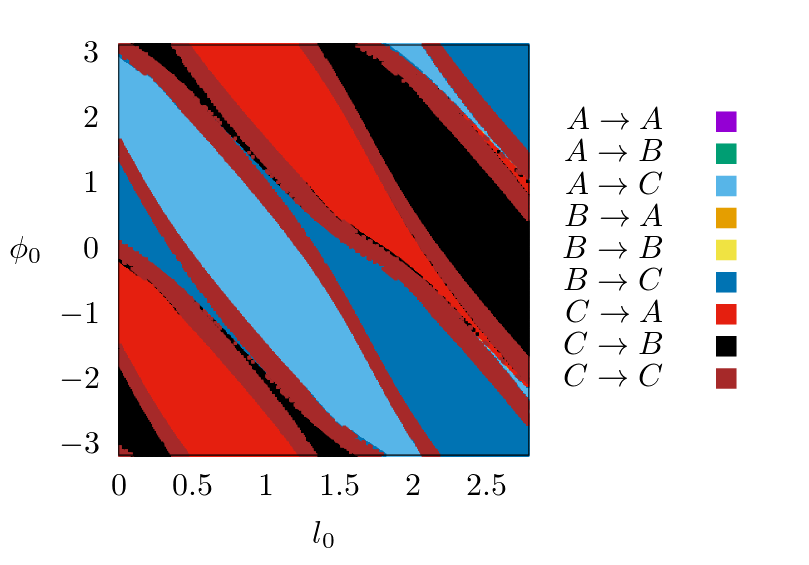
\includegraphics[scale=0.35]{fate_map_ds_gamma1E_0019.png}
	B)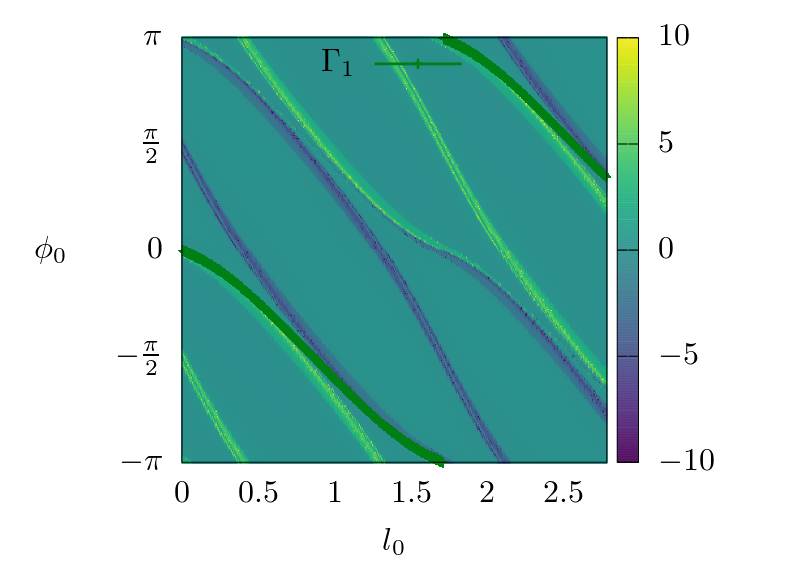
\includegraphics[scale=0.35]{ld_action_ds_gamma1_E_0019.png}
	C)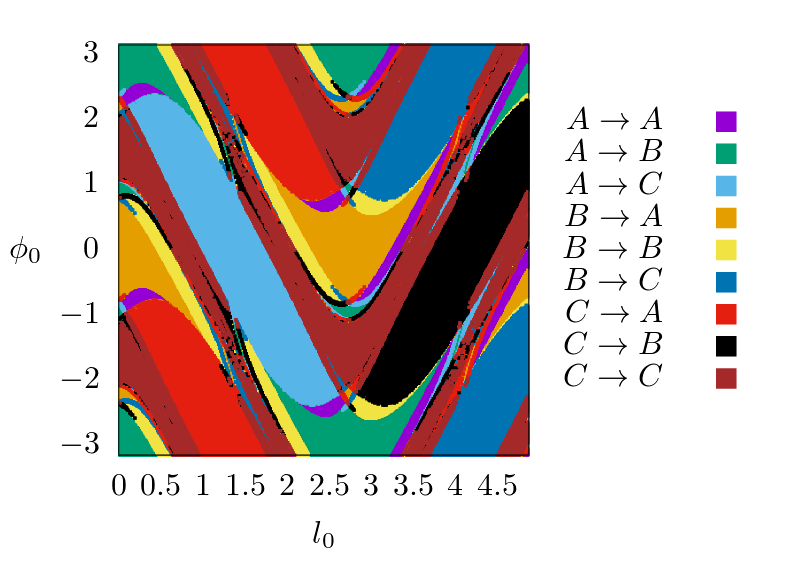
\includegraphics[scale=0.35]{fate_map_ds_gamma2E_0019.png}
	D)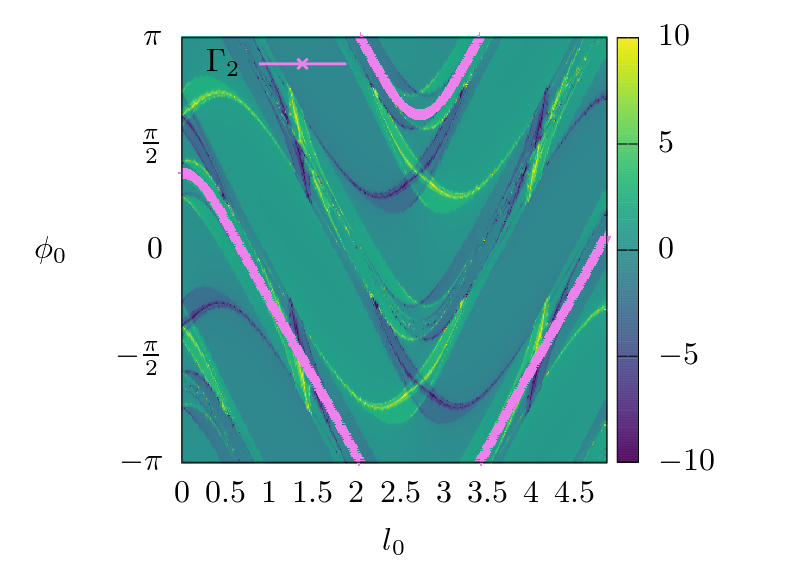
\includegraphics[scale=0.35]{ld_action_ds_gamma2_E_0019.png}
	E)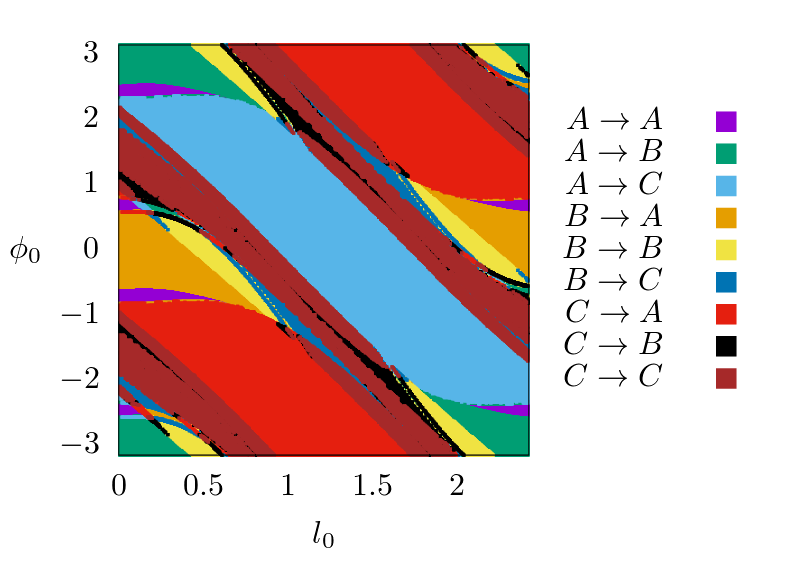
\includegraphics[scale=0.35]{fate_map_ds_gamma3E_0019.png}
	F)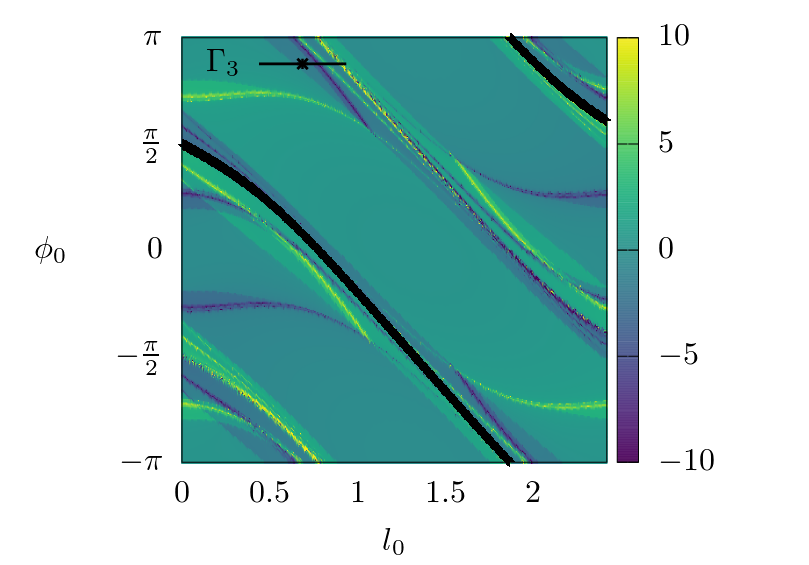
\includegraphics[scale=0.35]{ld_action_ds_gamma3_E_0019.png}
	\caption{ Fate maps and Lagrangian descriptors evaluated on the dividing surface corresponding to periodic orbits $\Gamma_1$, $\Gamma_2$, and $\Gamma_3$ for an energy before bifurcation of $\Gamma_3$ ($E$ =0.019). }
	\label{fig:ld_fm_ds_E_0019}
\end{figure}


\begin{figure}[htbp]
	A)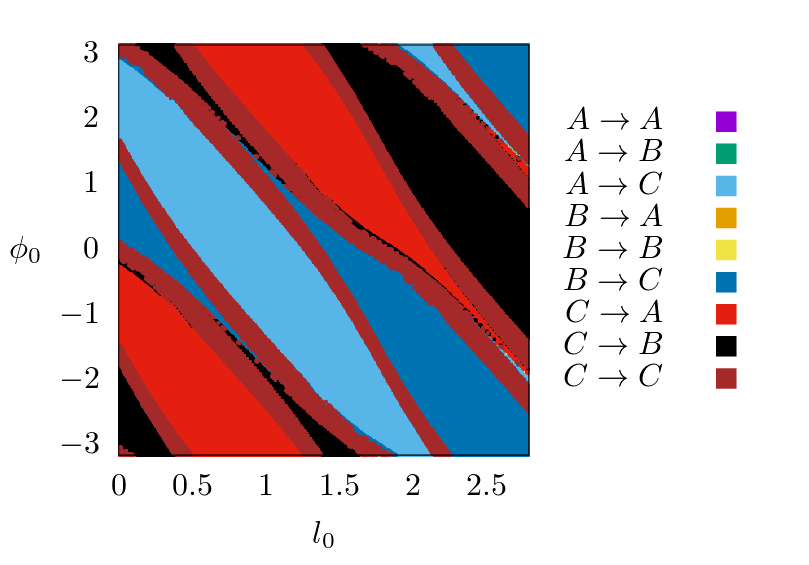
\includegraphics[scale=0.35]{fate_map_ds_gamma1E_0021.png}
	B)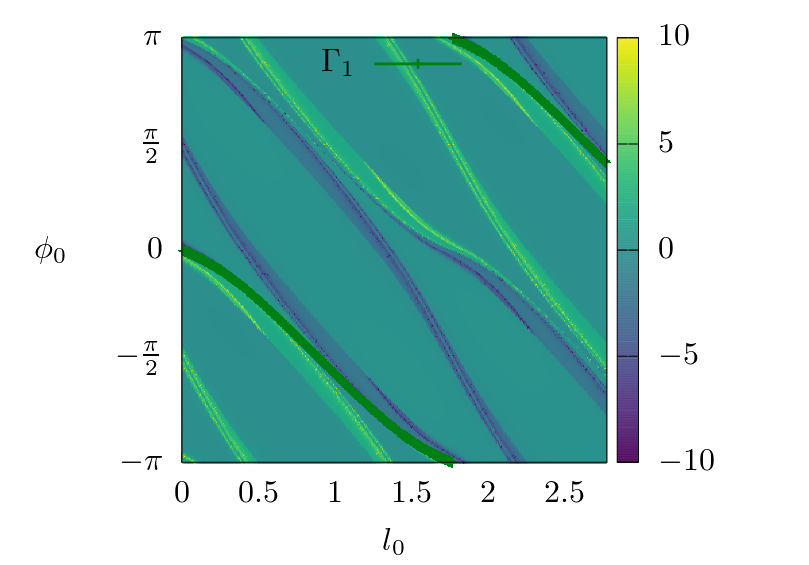
\includegraphics[scale=0.35]{ld_action_ds_gamma1_E_0021.png}
	C)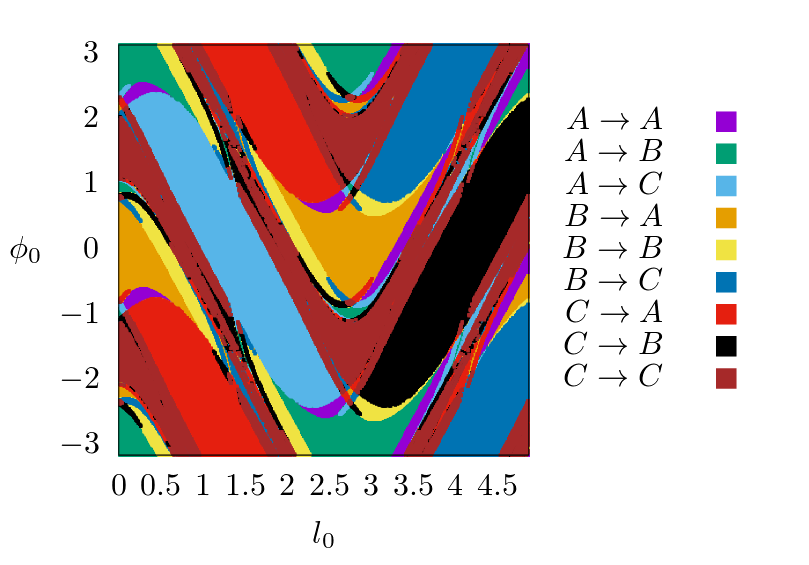
\includegraphics[scale=0.35]{fate_map_ds_gamma2E_0021.png}
	D)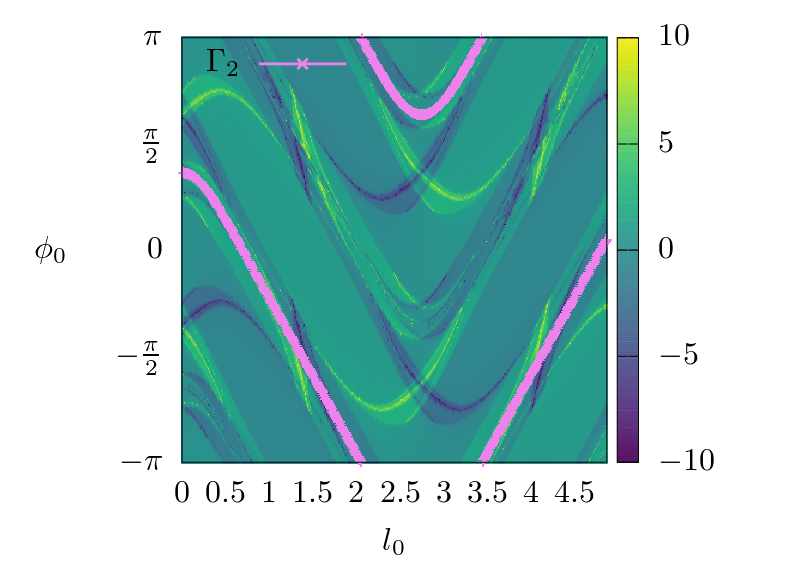
\includegraphics[scale=0.35]{ld_action_ds_gamma2_E_0021.png}
	\caption{ Fate maps and Lagrangian descriptors evaluated on the dividing surface corresponding to periodic orbits $\Gamma_1$ and $\Gamma_2$ for an energy after bifurcation of $\Gamma_3$  ($E$ =0.021). }
	\label{fig:ld_fm_ds_E_0021}
\end{figure}


\begin{figure}[htbp]
	A)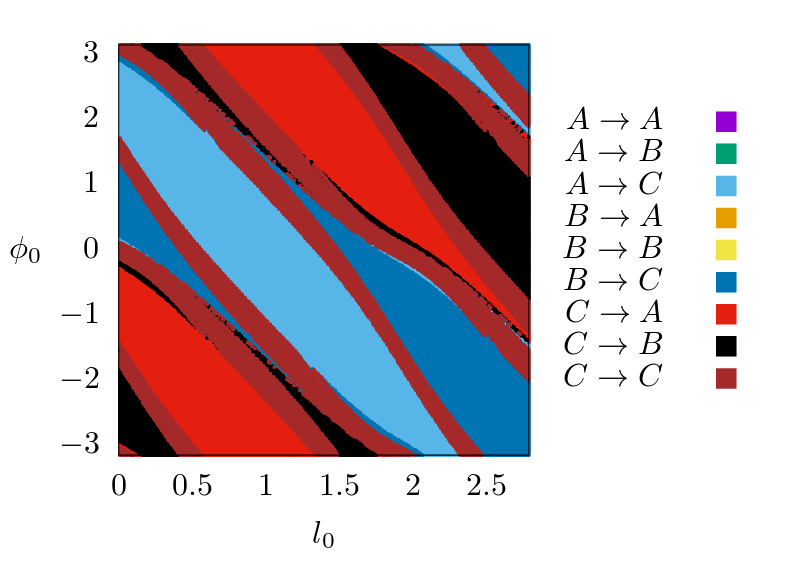
\includegraphics[scale=0.35]{fate_map_ds_gamma1E_0027.png}
	B)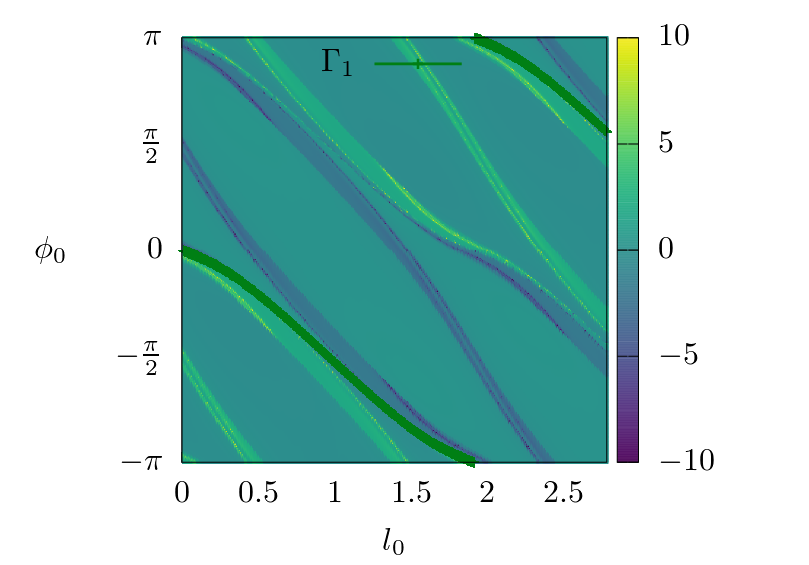
\includegraphics[scale=0.35]{ld_action_ds_gamma1_E_0027.png}
	C)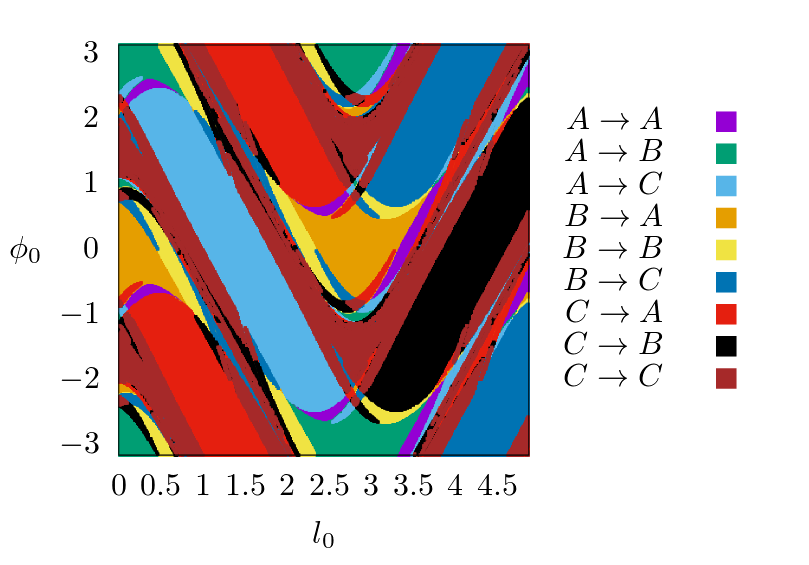
\includegraphics[scale=0.35]{fate_map_ds_gamma2E_0027.png}
	D)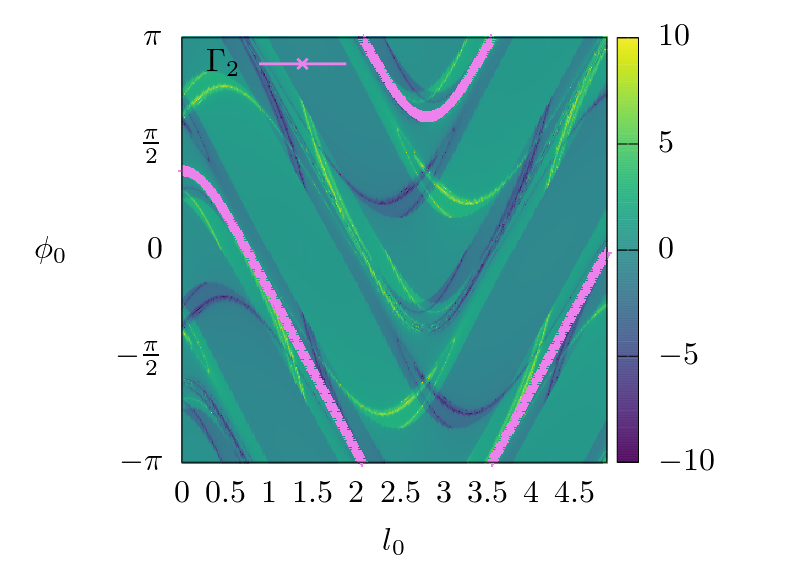
\includegraphics[scale=0.35]{ld_action_ds_gamma2_E_0027.png}
	\caption{ Fate maps and Lagrangian descriptors evaluated on the dividing surface corresponding to periodic orbits $\Gamma_1$ and $\Gamma_2$ for an energy before bifurcation of $\Gamma_2$    ($E$ =0.027). }
	\label{fig:ld_fm_ds_E_0027}
\end{figure}


\begin{figure}[htbp]
	A)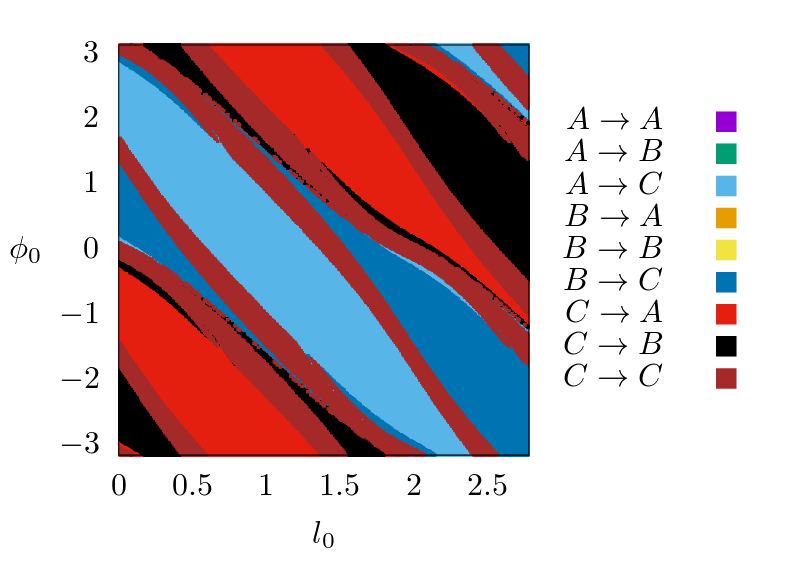
\includegraphics[scale=0.35]{fate_map_ds_gamma1E_003.png}
	B)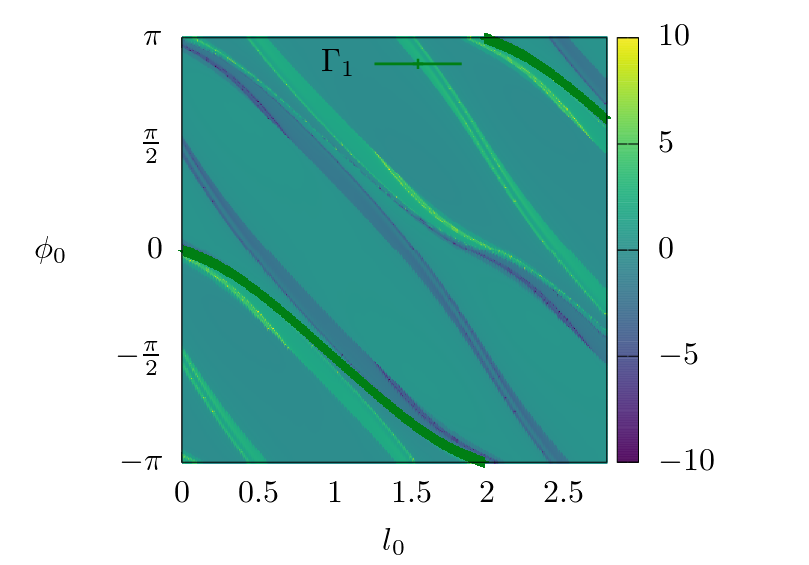
\includegraphics[scale=0.35]{ld_action_ds_gamma1_E_003.png}
	\caption{ Fate maps and Lagrangian descriptors evaluated on the dividing surface corresponding to periodic orbits $\Gamma_1$ and $\Gamma_2$ for an energy after bifurcation of $\Gamma_2$  ($E$ =0.03 ). }
	\label{fig:ld_fm_ds_E_003}
\end{figure}



\begin{figure}[htbp]
	A)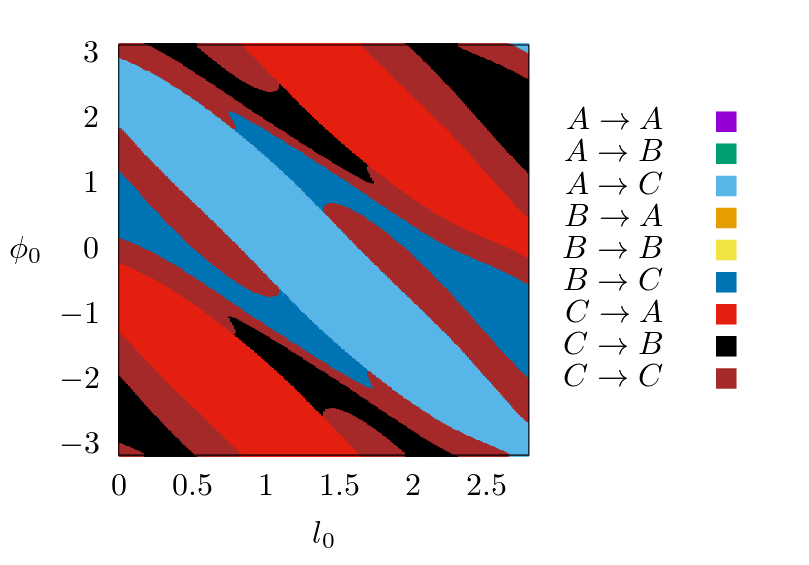
\includegraphics[scale=0.35]{fate_map_ds_gamma1E_0065.png}
	B)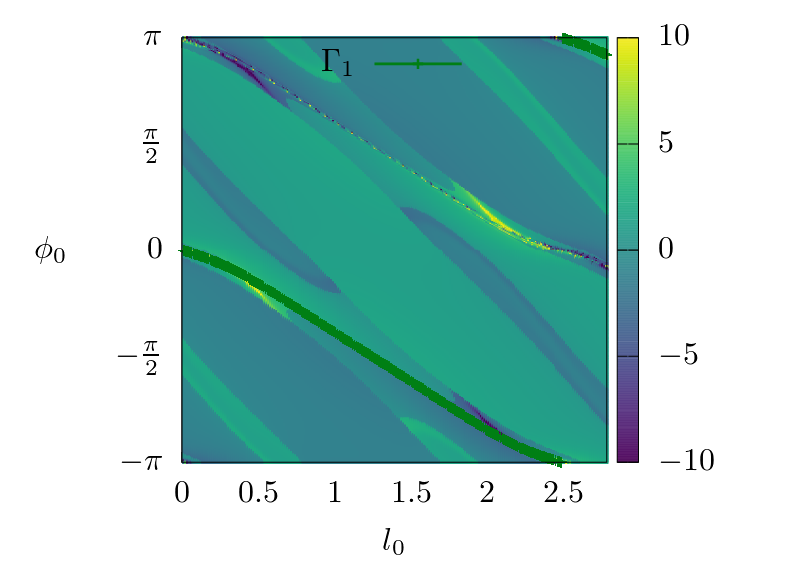
\includegraphics[scale=0.35]{ld_action_ds_gamma1_E_0065.png}
	\caption{ Fate maps and Lagrangian descriptors evaluated on the dividing surface corresponding to periodic orbit $\Gamma_1$ for an energy before bifurcation of $\Gamma_1$ ($E$ =0.065 ). }
	\label{fig:ld_fm_ds_E_0065}
\end{figure}


The figures show that the areas of the fate maps of the external periodic orbits do not change much after the bifurcation of the periodic orbits of the internal periodic orbits. For example let us consider the fate maps of the periodic orbits $\Gamma_1$ and $\Gamma_2$ after and before the bifurcation of the periodic orbit $\Gamma_3$, see figures \ref{fig:ld_fm_ds_E_0019} and \ref{fig:ld_fm_ds_E_0021}.  

\newpage

\subsection{other aspects}

\subsection{Bifurcation of the PES}

As shown in Figure \ref{fig:double_vdw_PES}C, the PES experiences a pitchfork bifurcation whenever $\eta = k/d  > \eta_c = \sqrt{7}$; where $k$ and $d$ are parameters in \eqref{eq:double_vdw}, and $\eta_c$ is the critical value of the bifurcation parameter. The system transitions from having three fixed points - an unstable saddle and two stable minima, to having a single stable minimum. This transition can be thought as the merging of the three original fixed points into one, as the height of the central barrier between the wells is lowered. 

%%%%%%%%%%%%%%%%%%%%%%%%%%%


\begin{figure}
    \centering
    A)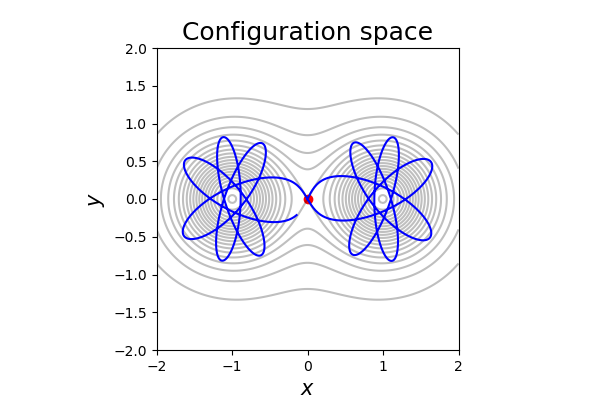
\includegraphics{traj_type2.png}
    B)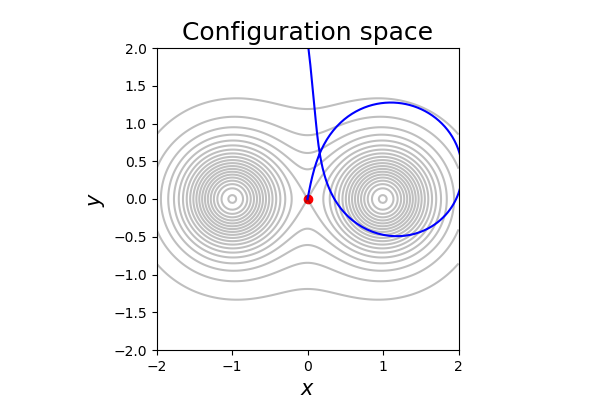
\includegraphics{traj_escapping.png}
    \caption{Example trajectories for bounding and dissociation energies, respectively. A) $E = -0.1$, B) $E=0.01$, with identical initial condition $(x_0, y_0) = (0, 0)$, and $p_{x,0} = 0.1$}
    \label{fig:my_label}
\end{figure}

%%%%%%%%%%%%%%%%%%%%%%%%%%%%%%%

\begin{figure}
    \centering
    A)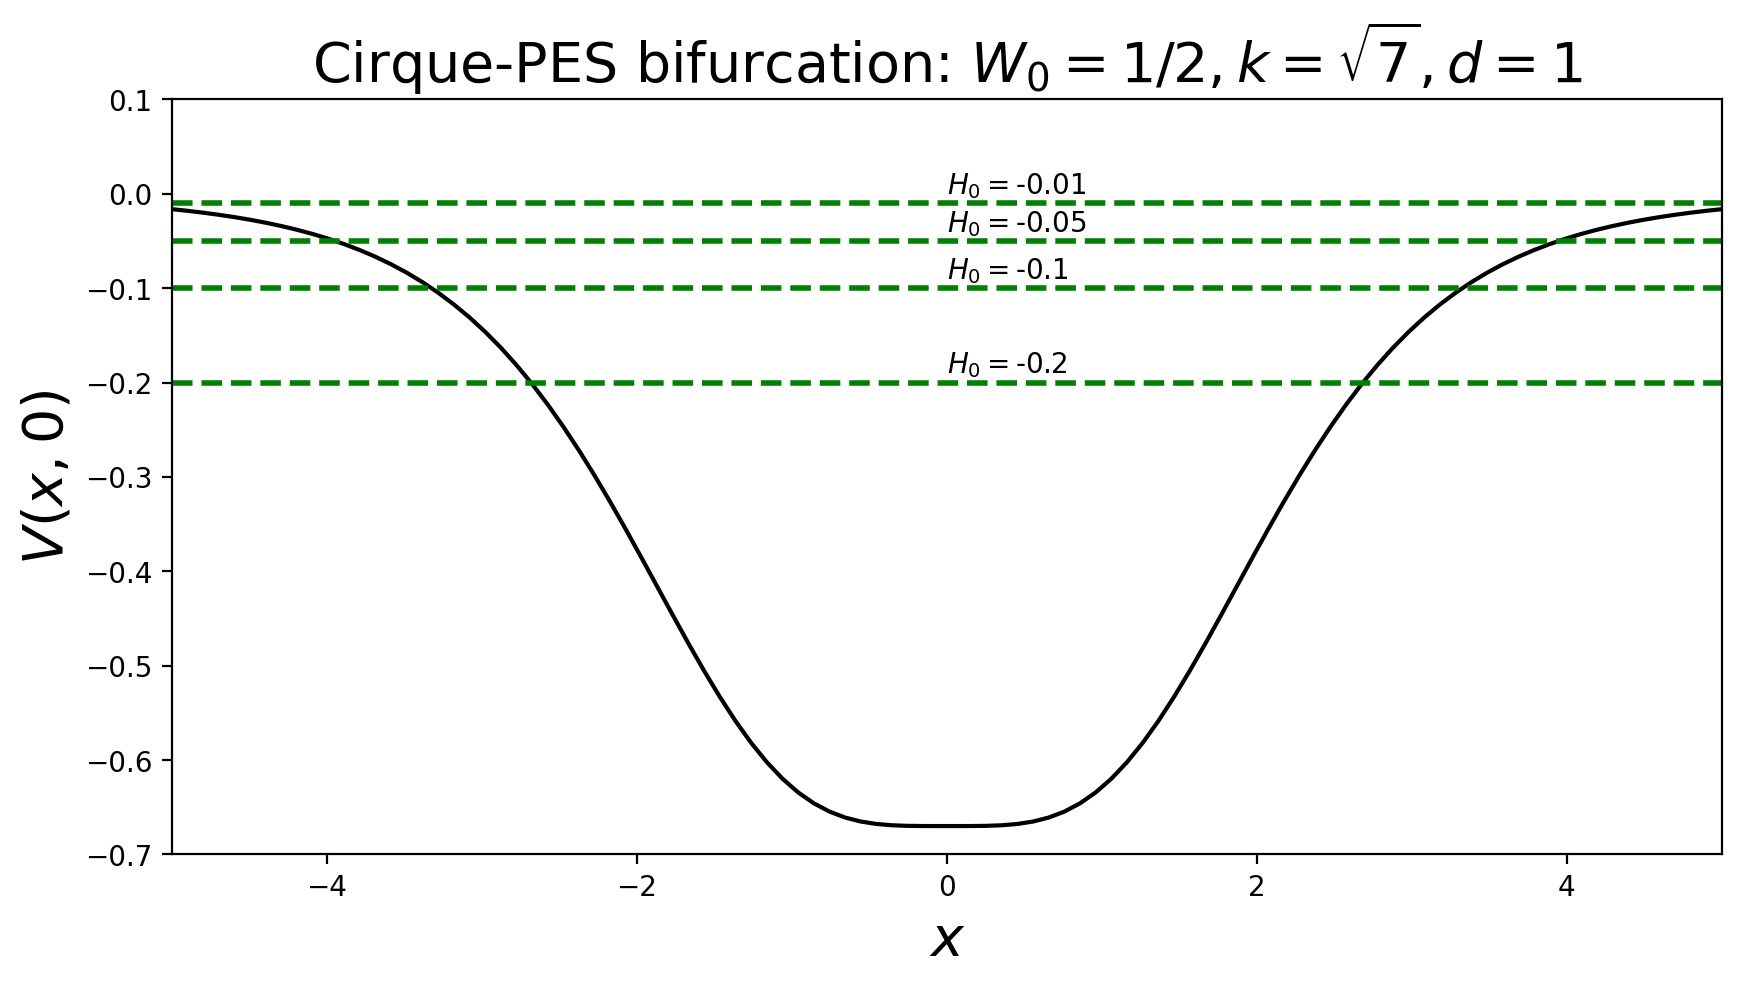
\includegraphics[width=0.45\textwidth]{pes_bifurcation_energy_levels.png}
    B)\includegraphics[width=0.45\textwidth]{pes_y_bifurcation_energy_levels.png}
    \caption{PES profile A) $y=0$; B) $x=0$; for critical bifurcation values and comparison with energy levels $H_0$}
\end{figure}

\begin{figure}[htbp]
	A)\includegraphics[scale=0.3]{PS_cirque_H_-0_2_y_0_w0_1div2_d_1_k_sqrt7.png}
	B)\includegraphics[scale=0.3]{PS_cirque_H_-0_1_y_0_w0_1div2_d_1_k_sqrt7.png}	
	C)\includegraphics[scale=0.3]{PS_cirque_H_-0_05_y_0_w0_1div2_d_1_k_sqrt7.png}
	D)\includegraphics[scale=0.3]{PS_cirque_H_-0_01_y_0_w0_1div2_d_1_k_sqrt7.png}
	\caption{Poincar\'e section $y = 0$ for the model parameters $W_0 = 1/2$, $k = \sqrt{7}$ and $d = 1$. The energy of the system is: A) $H_0 = -0.2$; B) $H_0 = -0.1$ ; C) $H_0 = -0.05$; D) $H_0 = -0.01$.}
	\label{fig:psec_y_0_bif}
\end{figure}

\begin{figure}
    \centering
    A) $H_0 = -0.2$ \includegraphics[width=0.6\textwidth]{notebooks/bifurcation/k_critical/LD_total_x-px_tau_500_k_kc_E_-0.4.png}\\
    A) $H_0 = -0.1$ \includegraphics[width=0.6\textwidth]{notebooks/bifurcation/k_critical/LD_total_x-px_tau_500_k_kc_E_-0.2.png}\\
    A) $H_0 = -0.05$ \includegraphics[width=0.6\textwidth]{notebooks/bifurcation/k_critical/LD_total_x-px_tau_500_k_kc_E_-0.1.png}\\
    A) $H_0 = -0.01$ \includegraphics[width=0.6\textwidth]{LD_total}
    \caption{LD maps for $x-p_x$ slices with model parameters $W_0 = 1/2$, $d = 1$, and $k = \sqrt{7}$ - critical value, with energy values under dissociation, $H_0 < 0$}
\end{figure}


\begin{figure}[htbp]
	A)\includegraphics[scale=0.3]{PS_cirque_H_-0_2_x_0_w0_1div2_d_1_k_sqrt7.png}
	B)\includegraphics[scale=0.3]{PS_cirque_H_-0_1_x_0_w0_1div2_d_1_k_sqrt7.png}	
	C)\includegraphics[scale=0.3]{PS_cirque_H_-0_05_x_0_w0_1div2_d_1_k_sqrt7.png}
	D)\includegraphics[scale=0.3]{PS_cirque_H_-0_01_x_0_w0_1div2_d_1_k_sqrt7.png}
	\caption{Poincar\'e section $x = 0$ for the model parameters $W_0 = 1/2$, $k = \sqrt{7}$ and $d = 1$. The energy of the system is: A) $H_0 = -0.2$; B) $H_0 = -0.1$ ; C) $H_0 = -0.05$; D) $H_0 = -0.01$.}
	\label{fig:psec_x_0_bif}
\end{figure}

\begin{figure}
    \centering
    A) $H_0 = -0.2$ \includegraphics[width=0.6\textwidth]{LD_H0_-0_2_y-py_PES_bifurcation.png}\\
    B) $H_0 = -0.1$ \includegraphics[width=0.6\textwidth]{LD_H0_-0_1_y-py_PES_bifurcation.png}\\
    C) $H_0 = -0.05$ \includegraphics[width=0.6\textwidth]{LD_H0_-0_05_y-py_PES_bifurcation.png}\\
    D) $H_0 = -0.01$ \includegraphics[width=0.6\textwidth]{LD_H0_-0_01_y-py_PES_bifurcation.png}
    \caption{LD maps for $y-p_y$ slices with model parameters $W_0 = 1/2$, $d = 1$, and $k = \sqrt{7}$ - critical value, with energy values under dissociation, $H_0 < 0$}
\end{figure}

\begin{figure}
    \centering
    \includegraphics{pes_profile_around_bifurcation.png}
    \caption{Caption}
\end{figure}


\begin{figure}
    \centering
    A) $k = \sqrt{7} -3 \delta$ \includegraphics[width=0.6\textwidth]{LD_H0_-0_2_x-px_PES_bifurcation_n_-3.png}\\
    B) $k = \sqrt{7} -2 \delta$ \includegraphics[width=0.6\textwidth]{LD_H0_-0_2_x-px_PES_bifurcation_n_-2.png}\\
    C) $k = \sqrt{7} - \delta$ \includegraphics[width=0.6\textwidth]{LD_H0_-0_2_x-px_PES_bifurcation_n_-1.png}\\
    D) $k = \sqrt{7}$ \includegraphics[width=0.6\textwidth]{LD_H0_-0_2_x-px_PES_bifurcation_n_0.png}
    \caption{LD maps for $x-p_x$ slices with model parameters $W_0 = 1/2$, $d = 1$, and $k = \sqrt{7} + n \delta$ with $\delta = 0.1$, below ($n < 0$) the critical bifurcation value ($n = 0$). The energy of the system is $H_0 = -0.2$}
\end{figure}


\begin{figure}
    \centering
    A) $k = \sqrt{7}$ \includegraphics[width=0.6\textwidth]{LD_H0_-0_2_x-px_PES_bifurcation_n_0.png}\\
    B) $k = \sqrt{7} + \delta$ \includegraphics[width=0.6\textwidth]{LD_H0_-0_2_x-px_PES_bifurcation_n_1.png}\\
    C) $k = \sqrt{7} + 2 \delta$ \includegraphics[width=0.6\textwidth]{LD_H0_-0_2_x-px_PES_bifurcation_n_2.png}\\
    D) $k = \sqrt{7} + 3 \delta$ \includegraphics[width=0.6\textwidth]{LD_H0_-0_2_x-px_PES_bifurcation_n_3.png}\\
    \caption{LD maps for $x-p_x$ slices with model parameters $W_0 = 1/2$, $d = 1$, and $k = \sqrt{7} + n \delta$ with $\delta = 0.1$, above ($n > 0$) the critical bifurcation value ($n = 0$). The energy of the system is $H_0 = -0.2$}
\end{figure}

\begin{figure}[htbp]
	A)\includegraphics[scale=0.3]{PS_y_0_H_-0_2_w0_1div2_k_sqrt7_min_5delta_d_1.png}
	B)\includegraphics[scale=0.3]{PS_y_0_H_-0_2_w0_1div2_k_sqrt7_min_4delta_d_1.png}	
	C)\includegraphics[scale=0.3]{PS_y_0_H_-0_2_w0_1div2_k_sqrt7_min_3delta_d_1.png}
	D)\includegraphics[scale=0.3]{PS_y_0_H_-0_2_w0_1div2_k_sqrt7_min_2delta_d_1.png}
	E)\includegraphics[scale=0.3]{PS_y_0_H_-0_2_w0_1div2_k_sqrt7_min_1delta_d_1.png}
	F)\includegraphics[scale=0.3]{PS_y_0_H_-0_2_w0_1div2_k_sqrt7_min_0delta_d_1.png}
	\caption{Poincar\'e section $y = 0$ for the model parameters $W_0 = 1/2$, $k = \sqrt{7} - \delta n$ and $d = 1$, where $\delta = 0.1$. The energy of the system is $H_0 = -0.2$. A) $n = 5$; B) $n = 4$; C) $n = 3$; D) $n = 2$; E) $n = 1$; F) $n = 0$.}
	\label{fig:psecBifProc_y_0}
\end{figure}

\begin{figure}[htbp]
	A)\includegraphics[scale=0.3]{PS_py_0_H_-0_2_w0_1div2_k_sqrt7_min_5delta_d_1.png}
	B)\includegraphics[scale=0.3]{PS_py_0_H_-0_2_w0_1div2_k_sqrt7_min_4delta_d_1.png}	
	C)\includegraphics[scale=0.3]{PS_py_0_H_-0_2_w0_1div2_k_sqrt7_min_3delta_d_1.png}
	D)\includegraphics[scale=0.3]{PS_py_0_H_-0_2_w0_1div2_k_sqrt7_min_2delta_d_1.png}
	E)\includegraphics[scale=0.3]{PS_py_0_H_-0_2_w0_1div2_k_sqrt7_min_1delta_d_1.png}
	F)\includegraphics[scale=0.3]{PS_py_0_H_-0_2_w0_1div2_k_sqrt7_min_0delta_d_1.png}
	\caption{Poincar\'e section $p_y = 0$ for the model parameters $W_0 = 1/2$, $k = \sqrt{7} - \delta n$ and $d = 1$, where $\delta = 0.1$. The energy of the system is $H_0 = -0.2$. A) $n = 5$; B) $n = 4$; C) $n = 3$; D) $n = 2$; E) $n = 1$; F) $n = 0$.}
	\label{fig:psecBifProc_py_0}
\end{figure}

\begin{figure}[htbp]
	A)\includegraphics[scale=0.3]{PS_px_0_H_-0_2_w0_1div2_k_sqrt7_min_5delta_d_1.png}
	B)\includegraphics[scale=0.3]{PS_px_0_H_-0_2_w0_1div2_k_sqrt7_min_4delta_d_1.png}	
	C)\includegraphics[scale=0.3]{PS_px_0_H_-0_2_w0_1div2_k_sqrt7_min_3delta_d_1.png}
	D)\includegraphics[scale=0.3]{PS_px_0_H_-0_2_w0_1div2_k_sqrt7_min_2delta_d_1.png}
	E)\includegraphics[scale=0.3]{PS_px_0_H_-0_2_w0_1div2_k_sqrt7_min_1delta_d_1.png}
	F)\includegraphics[scale=0.3]{PS_px_0_H_-0_2_w0_1div2_k_sqrt7_min_0delta_d_1.png}
	\caption{Poincar\'e section $p_x = 0$ for the model parameters $W_0 = 1/2$, $k = \sqrt{7} - \delta n$ and $d = 1$, where $\delta = 0.1$. The energy of the system is $H_0 = -0.2$. A) $n = 5$; B) $n = 4$; C) $n = 3$; D) $n = 2$; E) $n = 1$; F) $n = 0$.}
	\label{fig:psecBifProc_px_0}
\end{figure}


\section{Conclusions}
\label{sec:conclusion}



The dynamics associated with the roaming is present in this system and is similar to the dynamics of the double Morse system. For energies close to the threshold $E=0$, the fate maps have a similar structure that the fate maps and Lagrangian descriptor plots evaluated on the dividing surfaces corresponding to the double Morse potential system. This result is related to the nature of the potential energies outside the regions $A$ and $B$. Both potential energies have the same qualitative geometry outside those regions. The trajectories only travel a finite time before to reach the boundaries that divide the regions $A$, $B$, and $C$.
For this reason, the effects of the different geometrical features of both potentials are visible on the transport between the regions $A$, $B$, and $C$. The restricted dynamics are similar for both potentials energies.  
  


\section*{Acknowledgments}
The authors would like to acknowledge the financial support provided by the EPSRC Grant No. EP/P021123/1 and the Office of Naval Research Grant No. N00014-01-1-0769.

\bibliography{cirque}

\end{document}
